\documentclass[11pt,a4paper]{article}
\usepackage[margin=25mm]{geometry}
\usepackage{amsmath,amssymb}
\usepackage{graphicx}
\usepackage{hyperref}
\usepackage{booktabs}

\title{Machine Learning-based Prediction of Elastic Modulus in High-Entropy and Multi-Principal Element Alloys}
\author{Keisuke Nishioka (10081049)}
\date{2026-01-23}

\begin{document}

\maketitle

\begin{abstract}
The elastic modulus mismatch between metallic implants and human bone remains a central problem in biomedical materials design. High-entropy alloys (HEAs) and multi-principal element alloys (MPEAs) can, in principle, be tuned across a wide range of mechanical properties, but exploring their vast composition space experimentally is prohibitively costly. Here we compile elastic modulus data from multiple experimental and computational sources into a unified dataset of 5{,}339 alloys (roughly 6\% experimental, 94\% DFT-computed), spanning Young's modulus values from about 2.7~GPa to 621~GPa. From each alloy composition we derive 29 physically motivated features---composition fractions, atomic-radius and electronegativity statistics, valence electron concentration, and density---and use them to benchmark a range of regression models. An optimized SVR model reaches $R^2 \approx 0.59$ on a 322-sample dataset, and gradient boosting attains $R^2 \approx 0.67$ on an experimental-only subset. Feature-importance analyses consistently point to Ti content, average electronegativity, VEC, and density as dominant factors. We discuss implications for low-modulus HEA design targeting biomedical implants, as well as limitations of mixed experimental/computational data.
\end{abstract}

\section{Introduction}

Metallic implants such as hip and knee replacements must satisfy demanding mechanical and biological requirements. A particularly important issue is the elastic modulus mismatch between conventional metallic biomaterials (e.g., Ti--6Al--4V, Co--Cr alloys, stainless steels) and cortical bone. Human bone typically exhibits Young's modulus values in the range of roughly 10--30~GPa, while common metallic implant alloys often have moduli in the range of 100--200~GPa or higher. This mismatch can lead to stress shielding, bone resorption, and long-term implant loosening.

High-entropy alloys (HEAs) and multi-principal element alloys (MPEAs) have attracted growing interest as next-generation structural and functional materials \cite{Miracle2017}. Because they contain multiple principal elements in near-equimolar ratios, their mechanical properties---strength, ductility, corrosion resistance, and elastic modulus---can be tuned over a wide range. Refractory HEAs based on Ti, Zr, Nb, Ta, and Hf are of particular interest owing to their tunable stiffness \cite{Senkov2018}. For biomedical applications, alloys such as TiNbTaZrMo have been proposed as low-modulus implant candidates \cite{Todai2017}. The difficulty is that the composition--processing--property design space is enormous, and exhaustive experimental screening is impractical.

Several databases and studies have documented mechanical properties of HEAs and related alloys. The database by Gorsse \textit{et al.}\ \cite{Gorsse} compiles mechanical properties for HEAs and complex concentrated alloys, including Young's modulus for a large set of alloys. A DOE/OSTI dataset \cite{DOE} provides experimental Young's modulus values and related descriptors for high-entropy alloys. Large-scale computational databases such as the Materials Project \cite{MP} publish density-functional-theory (DFT) elastic tensors for inorganic compounds, from which bulk, shear, and Young's moduli can be derived. Recent reviews have also surveyed machine-learning approaches for HEA property prediction \cite{Wen2019}. Additional datasets, such as MPEA mechanical-property compilations and nano-indentation databases, further expand the available information.

In this project we bring these resources together into a single cleaned dataset and train machine-learning models to predict elastic modulus from composition-derived descriptors. An earlier phase focused on a 322-alloy experimental subset; here we report the full data pipeline and modeling results.

\begin{figure}[htbp]
\centering
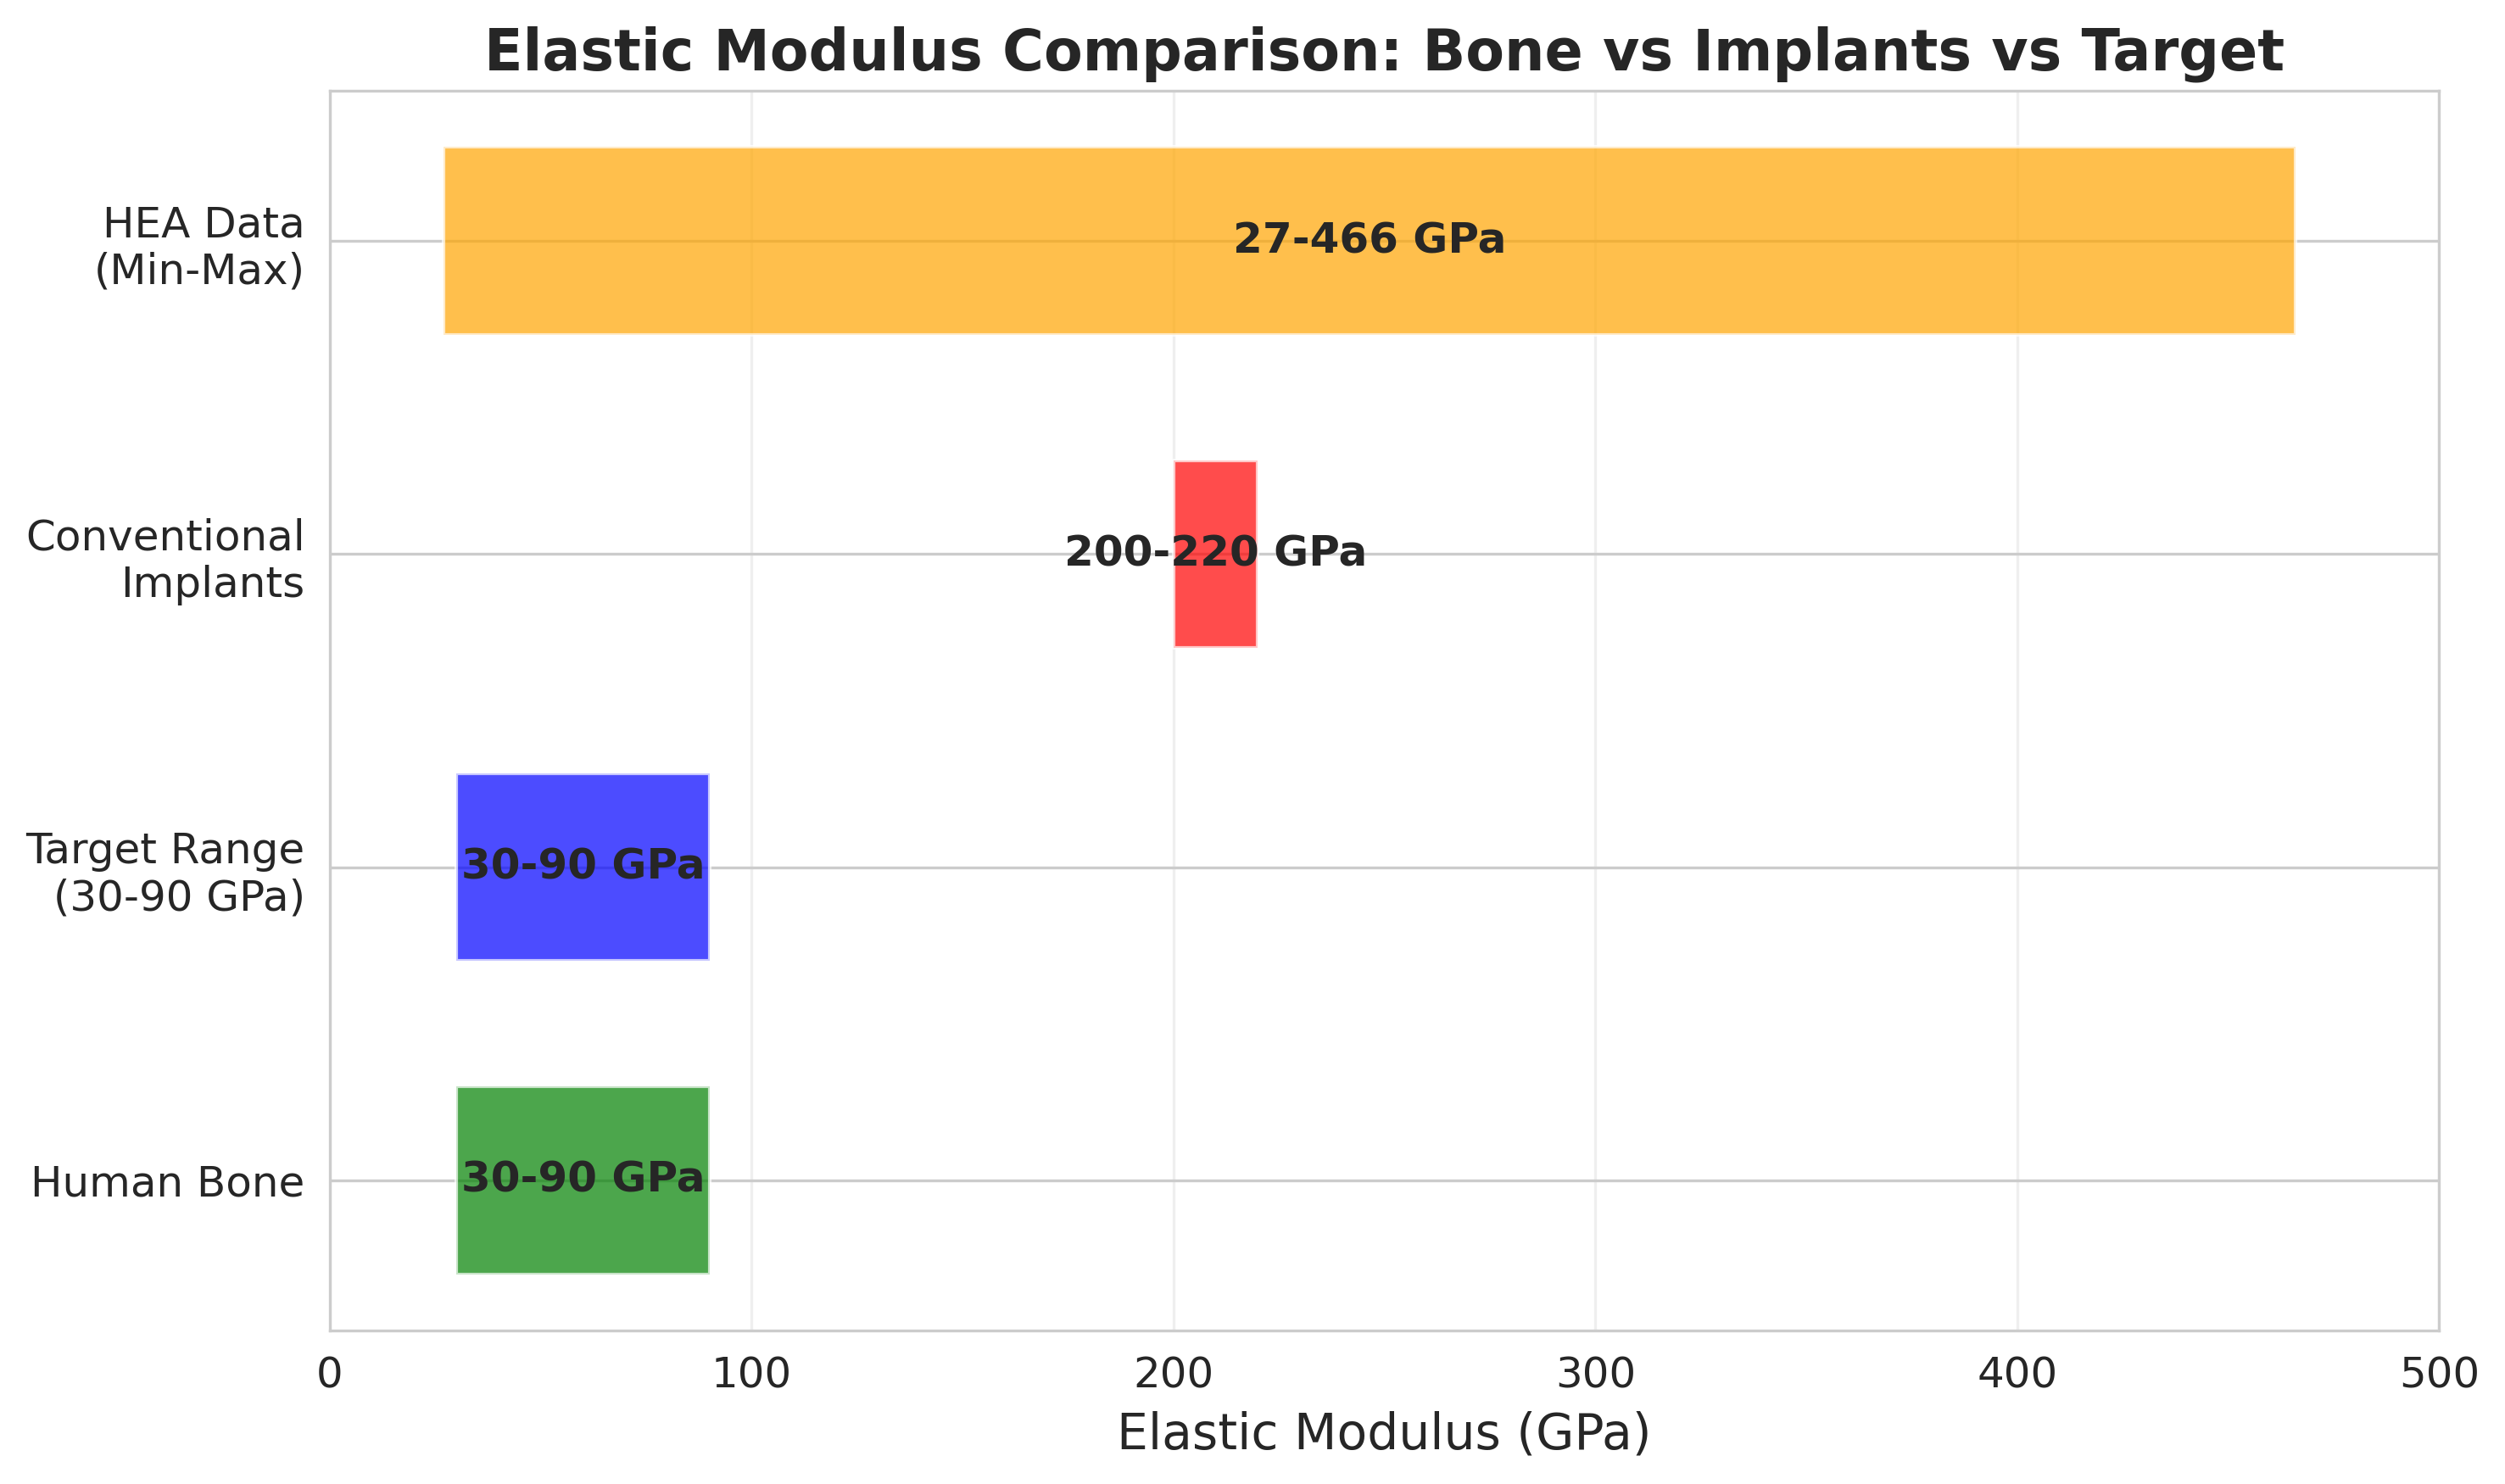
\includegraphics[width=0.85\textwidth]{figures/elastic_modulus_comparison.png}
\caption{Comparison of elastic modulus ranges for human bone, conventional metallic biomaterials, and target range for biomedical HEA/MPEA alloys. The mismatch between bone (10--30~GPa) and traditional implants (100--200~GPa) motivates the design of low-modulus alloys in the 30--90~GPa range.}
\label{fig:elastic_modulus_comparison}
\end{figure}

\section{Data and Dataset Construction}

\subsection{Data Sources}

The final integrated dataset is constructed from a combination of experimental and computational sources:

\begin{itemize}
  \item \textbf{DOE/OSTI HEA dataset (experimental)}: A curated dataset of high-entropy alloys with phase information and experimentally measured Young's modulus for a subset of alloys. After de-duplication and cleaning, 101 alloys with valid modulus values are retained.
  \item \textbf{Gorsse HEA mechanical-properties database (experimental)}: A literature-based database of HEAs and complex concentrated alloys with composition, microstructure, density, hardness, strength, elongation, and Young's modulus. We include 182 unique alloys with valid Young's modulus.
  \item \textbf{Latest experimental HEA data}: Additional data from recent publications on Ti--Zr--Nb, Ti--Zr--Hf--Nb--Ta, and related biocompatible HEA/MPEA systems. Due to overlaps with earlier databases and nano-indentation compilations, the net increase in unique alloys is modest.
  \item \textbf{MPEA nano-indentation dataset (experimental and computed)}: A dataset of phase-specific mechanical properties measured by nano-indentation in multi-principal element alloys. From this dataset, we extract 51 experimental entries and 196 calculated entries with Young's modulus after integration.
  \item \textbf{Refractory HEA elastic-constants dataset (computed)}: A set of DFT-computed elastic constants for 370 refractory HEAs, from which Young's modulus is derived.
  \item \textbf{Materials Project (computed)}: DFT-derived elastic tensors for a large number of inorganic compounds. For suitable compositions related to HEA/MPEA chemistries, Young's modulus is computed via
  \begin{equation}
    E = \frac{9KG}{3K + G},
  \end{equation}
  where $K$ and $G$ are bulk and shear moduli, respectively. This source contributes 4{,}439 samples.
\end{itemize}

Auxiliary databases such as DISMA and MPEA mechanical-property compilations are used for cross-checking and metadata but are not primary sources for the target property.

\subsection{Integration and Cleaning}

Each dataset is first parsed into a standardized tabular format with at least an alloy identifier, Young's modulus in GPa, and a source label. The main integration steps are:

\begin{enumerate}
  \item Column harmonization to a unified label \texttt{elastic\_modulus} in GPa;
  \item Removal of entries with missing, non-positive, or clearly unphysical modulus values;
  \item Duplicate detection and removal based on alloy name, composition, and modulus;
  \item Enforcement of mandatory fields (\texttt{alloy\_name}, \texttt{elastic\_modulus}, \texttt{source});
  \item Validation of the final table using dedicated scripts that check schema consistency, missing values, duplicates, and basic statistics.
\end{enumerate}

The final cleaned dataset is stored as \texttt{unified\_dataset\_cleaned\_20260123\_175245.csv} (with a stable copy \texttt{unified\_dataset\_latest.csv}) and contains 5{,}339 unique alloy entries.

\subsection{Dataset Characteristics}

The 5{,}339-sample integrated dataset has the following key attributes:

\begin{itemize}
  \item Source breakdown:
    \begin{itemize}
      \item Materials Project: 4{,}439 samples (83.1\%);
      \item Refractory HEA elastic constants: 370 samples (6.9\%);
      \item MPEA nano-indentation (calculated): 196 samples (3.7\%);
      \item Gorsse database: 182 samples (3.4\%);
      \item DOE/OSTI: 101 samples (1.9\%);
      \item MPEA nano-indentation (experimental): 51 samples (1.0\%).
    \end{itemize}
  \item Experimental vs.\ computed:
    \begin{itemize}
      \item Experimental Young's modulus: 335 samples ($\approx 6.3$\%);
      \item Computed Young's modulus: 5{,}004 samples ($\approx 93.7$\%).
    \end{itemize}
  \item Young's modulus distribution:
    \begin{itemize}
      \item Minimum: 2.73~GPa;
      \item Maximum: 621.33~GPa;
      \item Mean: 139.26~GPa;
      \item Median: 122.61~GPa.
    \end{itemize}
\end{itemize}

An earlier phase of the project used a predominantly experimental subset of 322 alloys (from DOE/OSTI, Gorsse, and recent experiments) for model development. In that subset, Young's modulus ranges approximately from 27--466~GPa, with about 30 alloys in the 30--90~GPa range relevant for bone-like stiffness.

\begin{figure}[htbp]
\centering
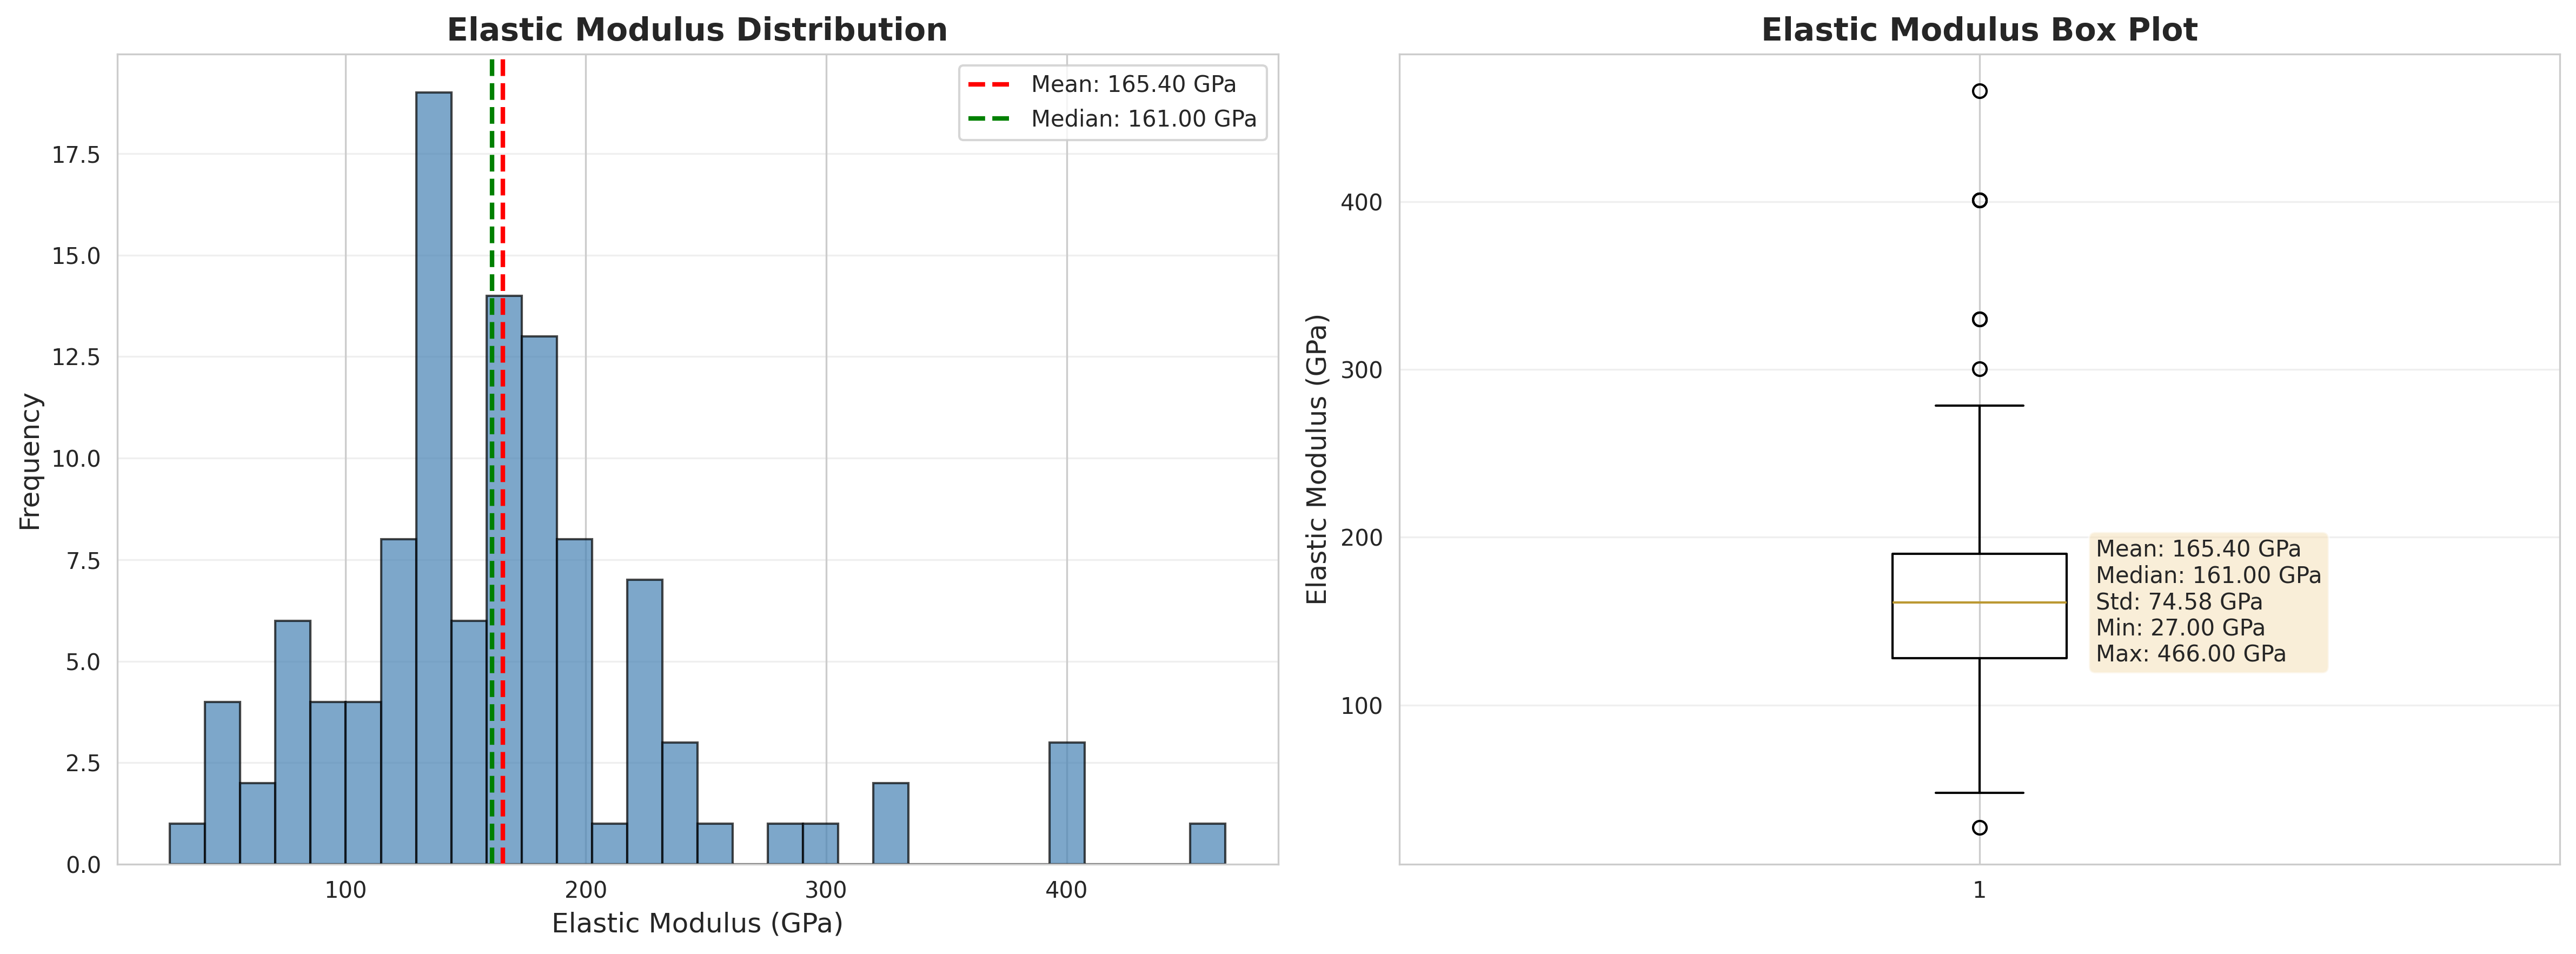
\includegraphics[width=0.85\textwidth]{figures/data_distribution.png}
\caption{Distribution of elastic modulus values in the integrated dataset (5{,}339 samples). The histogram shows a broad distribution spanning from approximately 2.7~GPa to 621~GPa, with a mean around 139~GPa. The target range for biomedical applications (30--90~GPa) is highlighted.}
\label{fig:data_distribution}
\end{figure}

\begin{figure}[htbp]
\centering
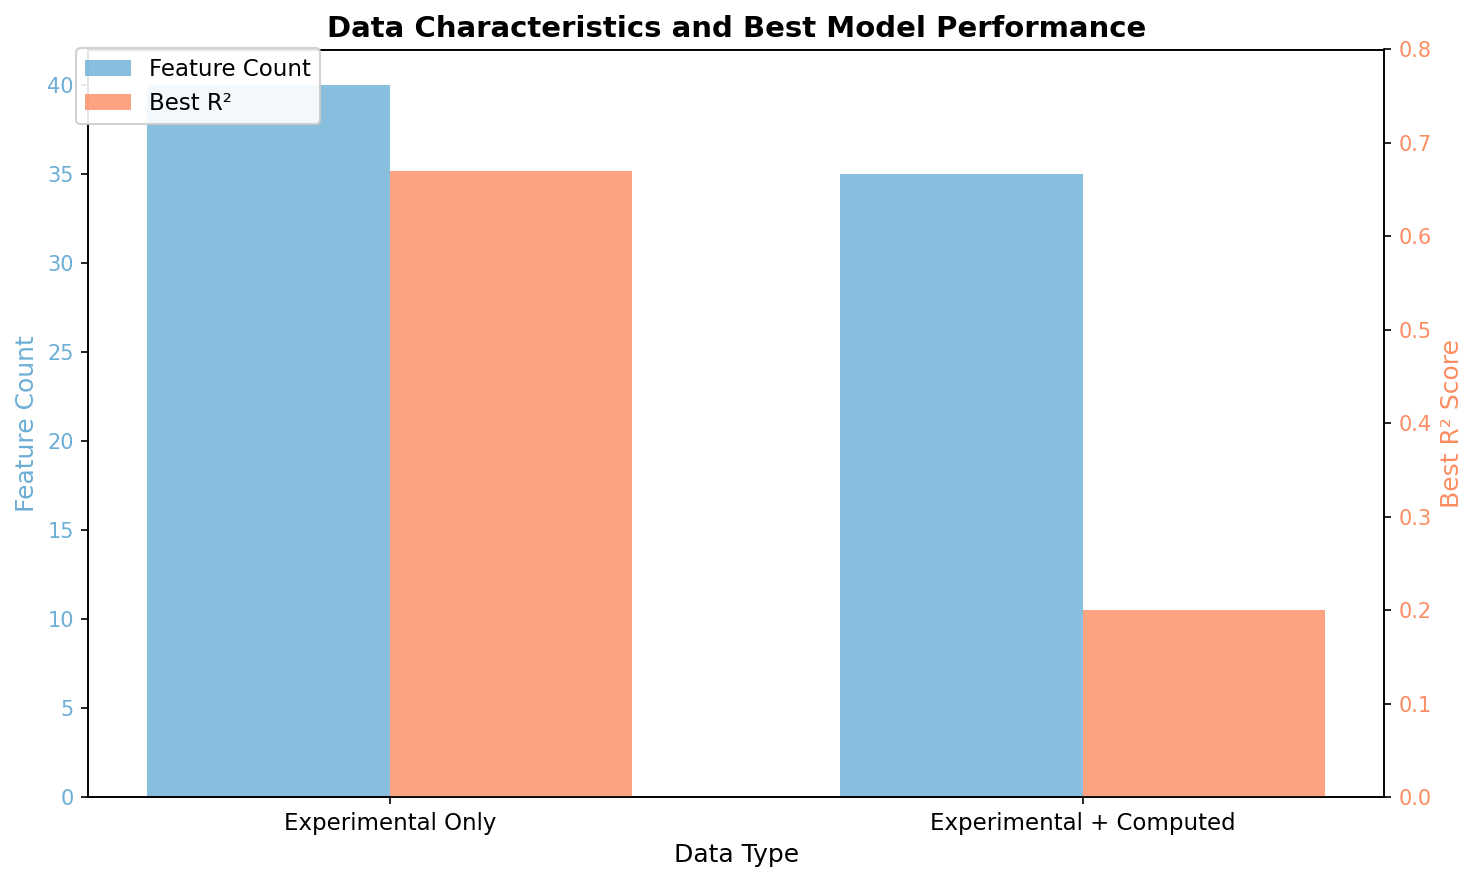
\includegraphics[width=0.85\textwidth]{figures/data_characteristics.png}
\caption{Key characteristics of the integrated dataset, including source breakdown, experimental vs.\ computed data distribution, and statistical properties of the elastic modulus values.}
\label{fig:data_characteristics}
\end{figure}

\section{Features and Machine Learning Methods}

\subsection{Feature Engineering}

Following established feature engineering practices for materials informatics \cite{Ward2016}, we construct 29 features combining composition information with atomic and thermodynamic descriptors. The main categories are:

\begin{itemize}
  \item Atomic-radius descriptors: average, standard deviation, maximum, minimum, and spread of atomic radius;
  \item Electronegativity descriptors: average, standard deviation, and spread of electronegativity;
  \item Electronic/thermodynamic descriptors: valence electron concentration (VEC), configurational mixing entropy, and number of elements;
  \item Composition fractions for 17 elements: Ti, Zr, Hf, Nb, Ta, V, Cr, Mo, W, Fe, Co, Ni, Cu, Al, Mn, Si, Sn;
  \item Additional physical descriptors: density and selected dataset-specific quantities.
\end{itemize}

\subsection{Models and Training Protocol}

We benchmark linear models (ordinary least squares, Ridge, Lasso), polynomial regression, K-nearest neighbors, random forest \cite{Breiman2001}, gradient boosting \cite{ChenGuestrin2016}, stacking ensembles, support vector regression (SVR) \cite{Vapnik1995}, and a feedforward neural network. Beyond these classical methods, we also train several deep-learning architectures: Fourier Neural Operators (FNO) \cite{Li2021FNO}, DeepONet \cite{Lu2021}, MEGNet \cite{Chen2019MEGNet}, CGCNN \cite{Xie2018}, a custom graph neural network (HEAGNN), physics-informed neural networks (PINNs) \cite{Raissi2019}, Neural ODEs, and a composition-based Transformer (HEATransformer) following the self-attention framework of Vaswani et al.\ \cite{Vaswani2017}. The deep-learning models are implemented in the \texttt{fno\_models} and \texttt{gnn\_transformer\_models} modules. All models use an 80/20 train/test split; hyperparameters are tuned via 5-fold cross-validation. We report the coefficient of determination $R^2$, root mean squared error (RMSE), and mean absolute error (MAE).

\begin{figure}[htbp]
\centering
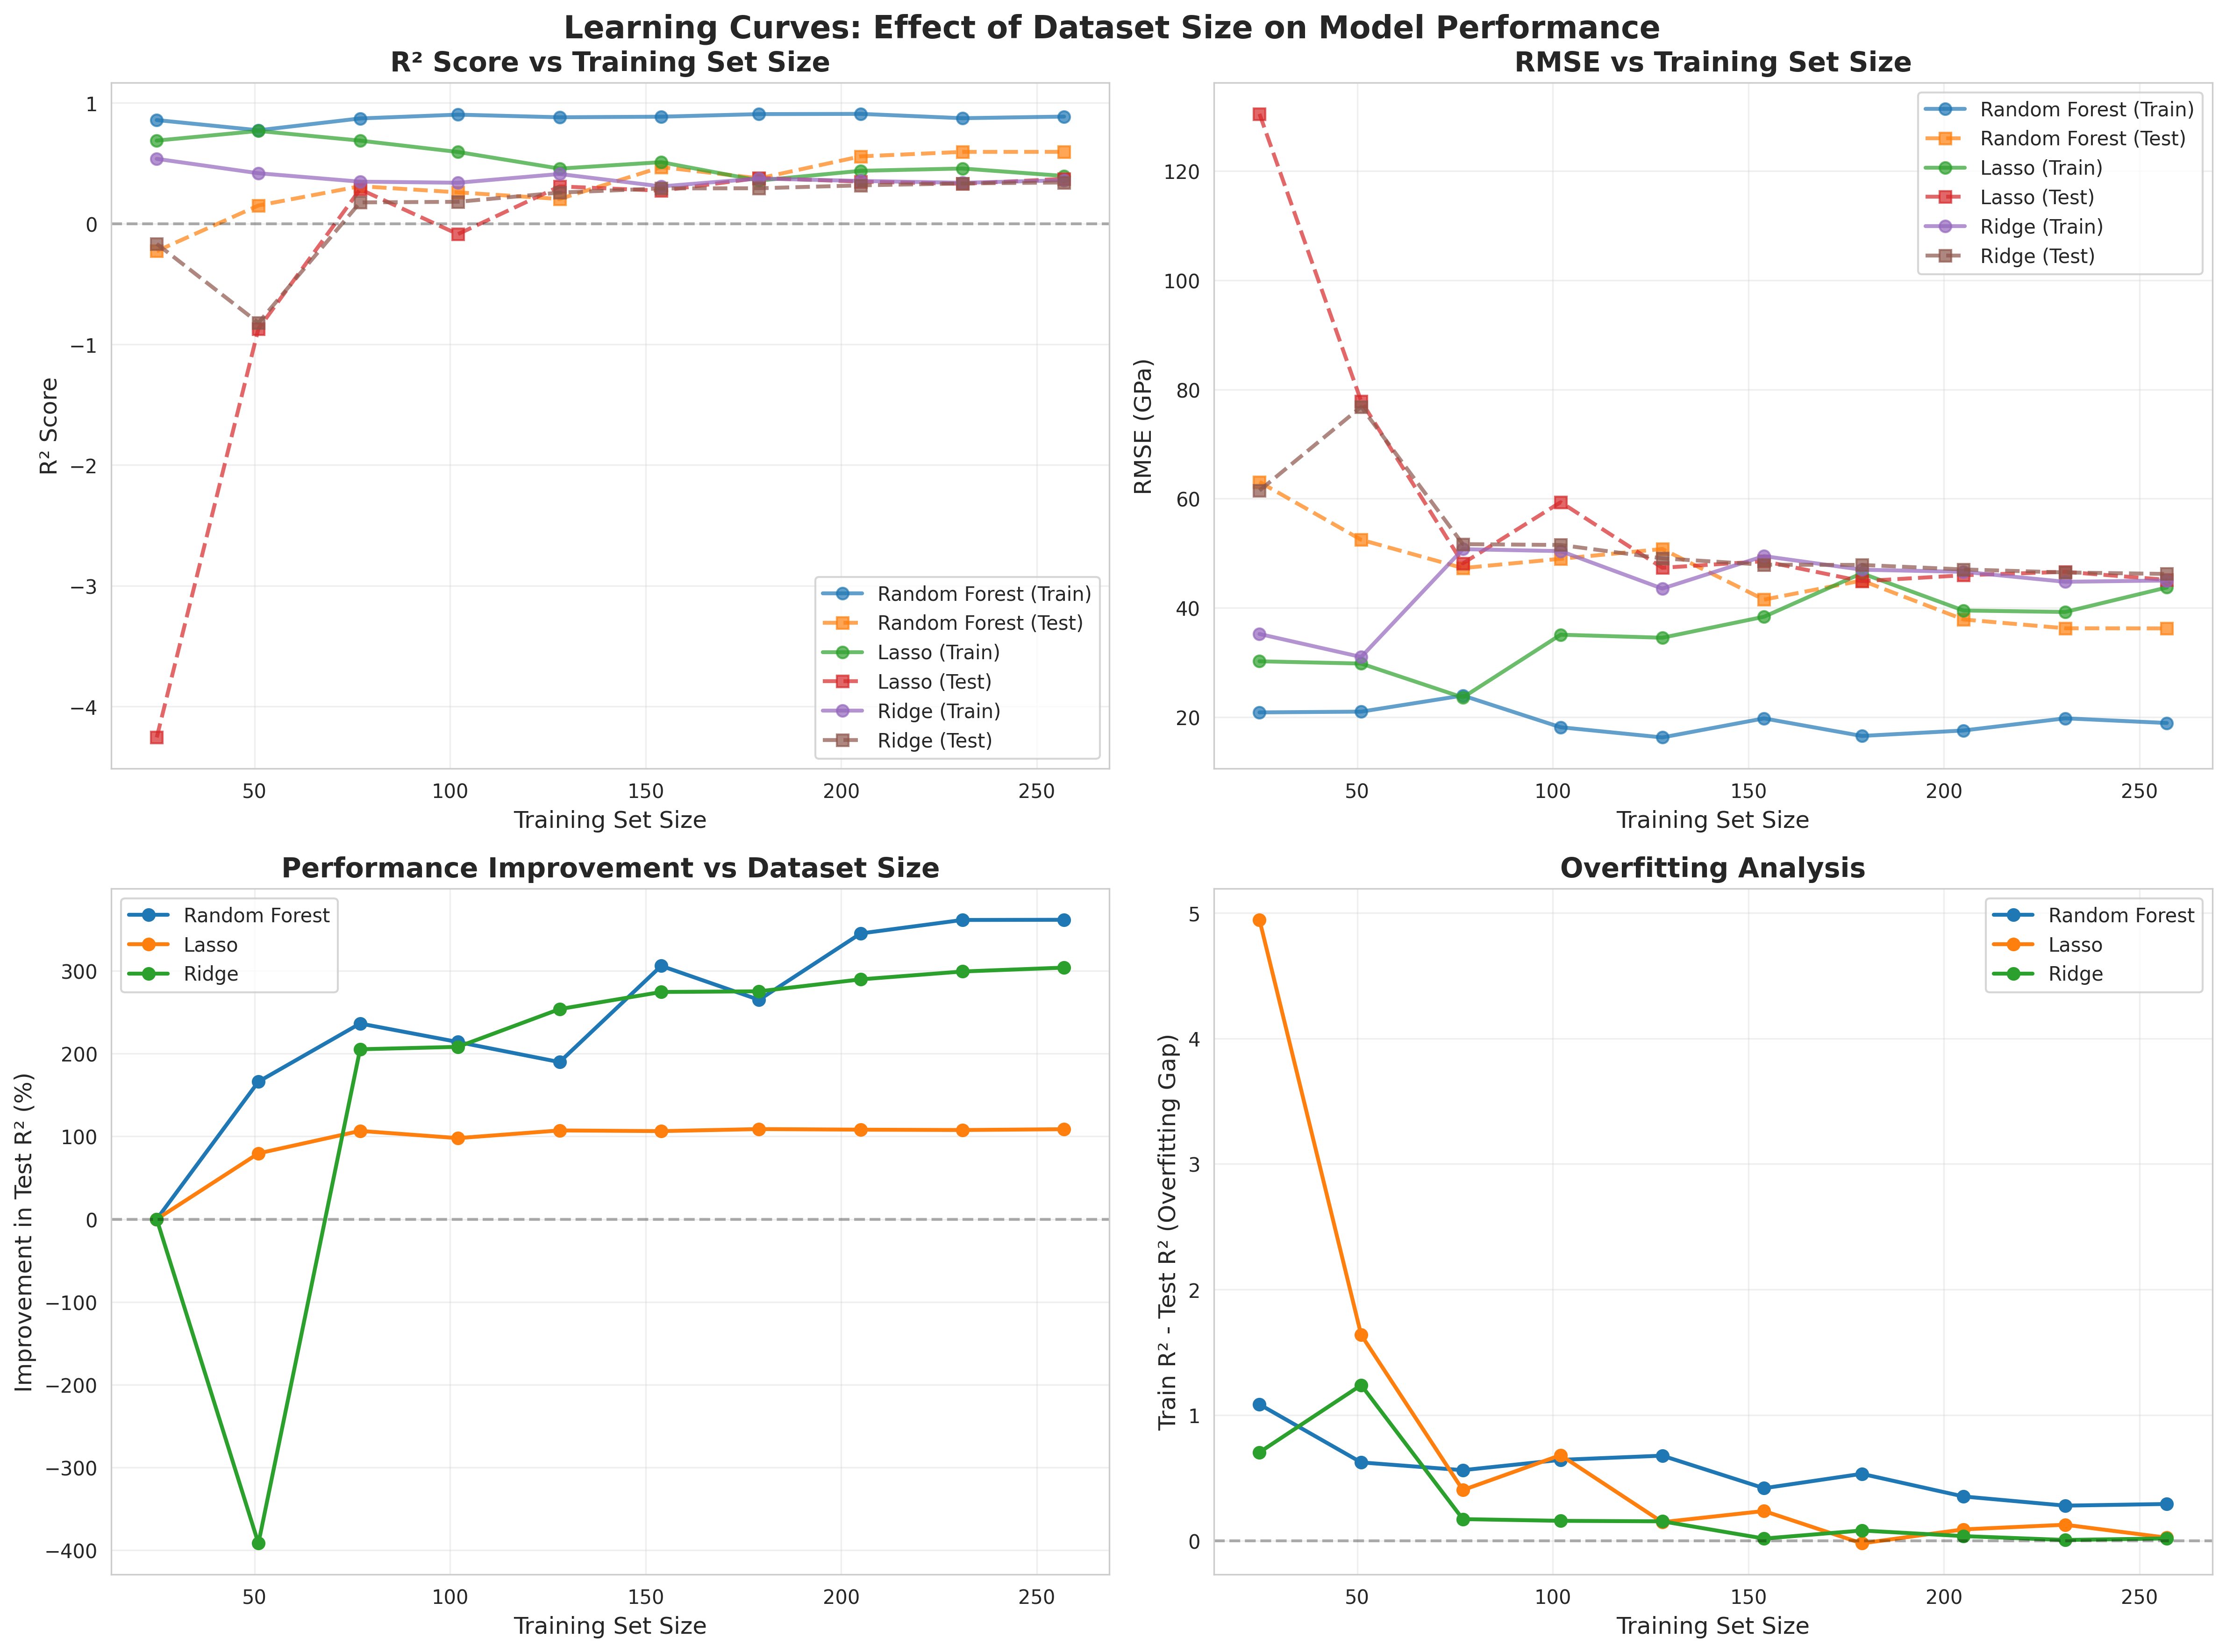
\includegraphics[width=0.85\textwidth]{figures/learning_curves.png}
\caption{Learning curves showing training and validation performance over epochs for selected models. The curves demonstrate convergence behavior and help identify optimal stopping points to prevent overfitting.}
\label{fig:learning_curves}
\end{figure}

\section{Results and Discussion}

On the 322-sample dataset, random forest gives the best untuned result ($R^2 \approx 0.57$, RMSE $\approx$ 37.5~GPa). After hyperparameter optimization SVR reaches $R^2 \approx 0.59$ (RMSE $\approx$ 36.2~GPa). On an experimental-only subset of roughly 109 samples, gradient boosting achieves $R^2 \approx 0.67$---a reasonable result given the limited and heterogeneous data. The HEATransformer obtains $R^2 \approx 0.62$ (RMSE 34.9~GPa, MAE 26.2~GPa) on the 322-sample set, suggesting that self-attention over composition tokens can capture useful compositional patterns.

\begin{table}[htbp]
\centering
\caption{Model performance comparison on the 322-sample experimental dataset. Performance metrics include coefficient of determination ($R^2$), root mean squared error (RMSE), and mean absolute error (MAE).}
\label{tab:model_performance}
\begin{tabular}{lccc}
\hline
Model & Test $R^2$ & Test RMSE (GPa) & Test MAE (GPa) \\
\hline
Random Forest & 0.57 & 37.5 & 25.9 \\
SVR (optimized) & 0.59 & 36.2 & 24.8 \\
Gradient Boosting (exp.\ only) & 0.67 & 49.7 & 37.1 \\
MLFFNN & 0.49 & 40.5 & 29.0 \\
Lasso & 0.37 & 45.1 & 31.3 \\
Linear & 0.36 & 45.5 & 32.6 \\
SVR (baseline) & 0.36 & 45.6 & 29.1 \\
Ridge & 0.34 & 46.2 & 32.0 \\
KNN & 0.02 & 56.3 & 44.4 \\
Polynomial & $<$0 & 97.5 & 61.1 \\
Transformer (HEATransformer) & 0.62 & 34.9 & 26.2 \\
\hline
\end{tabular}
\end{table}

\begin{figure}[htbp]
\centering
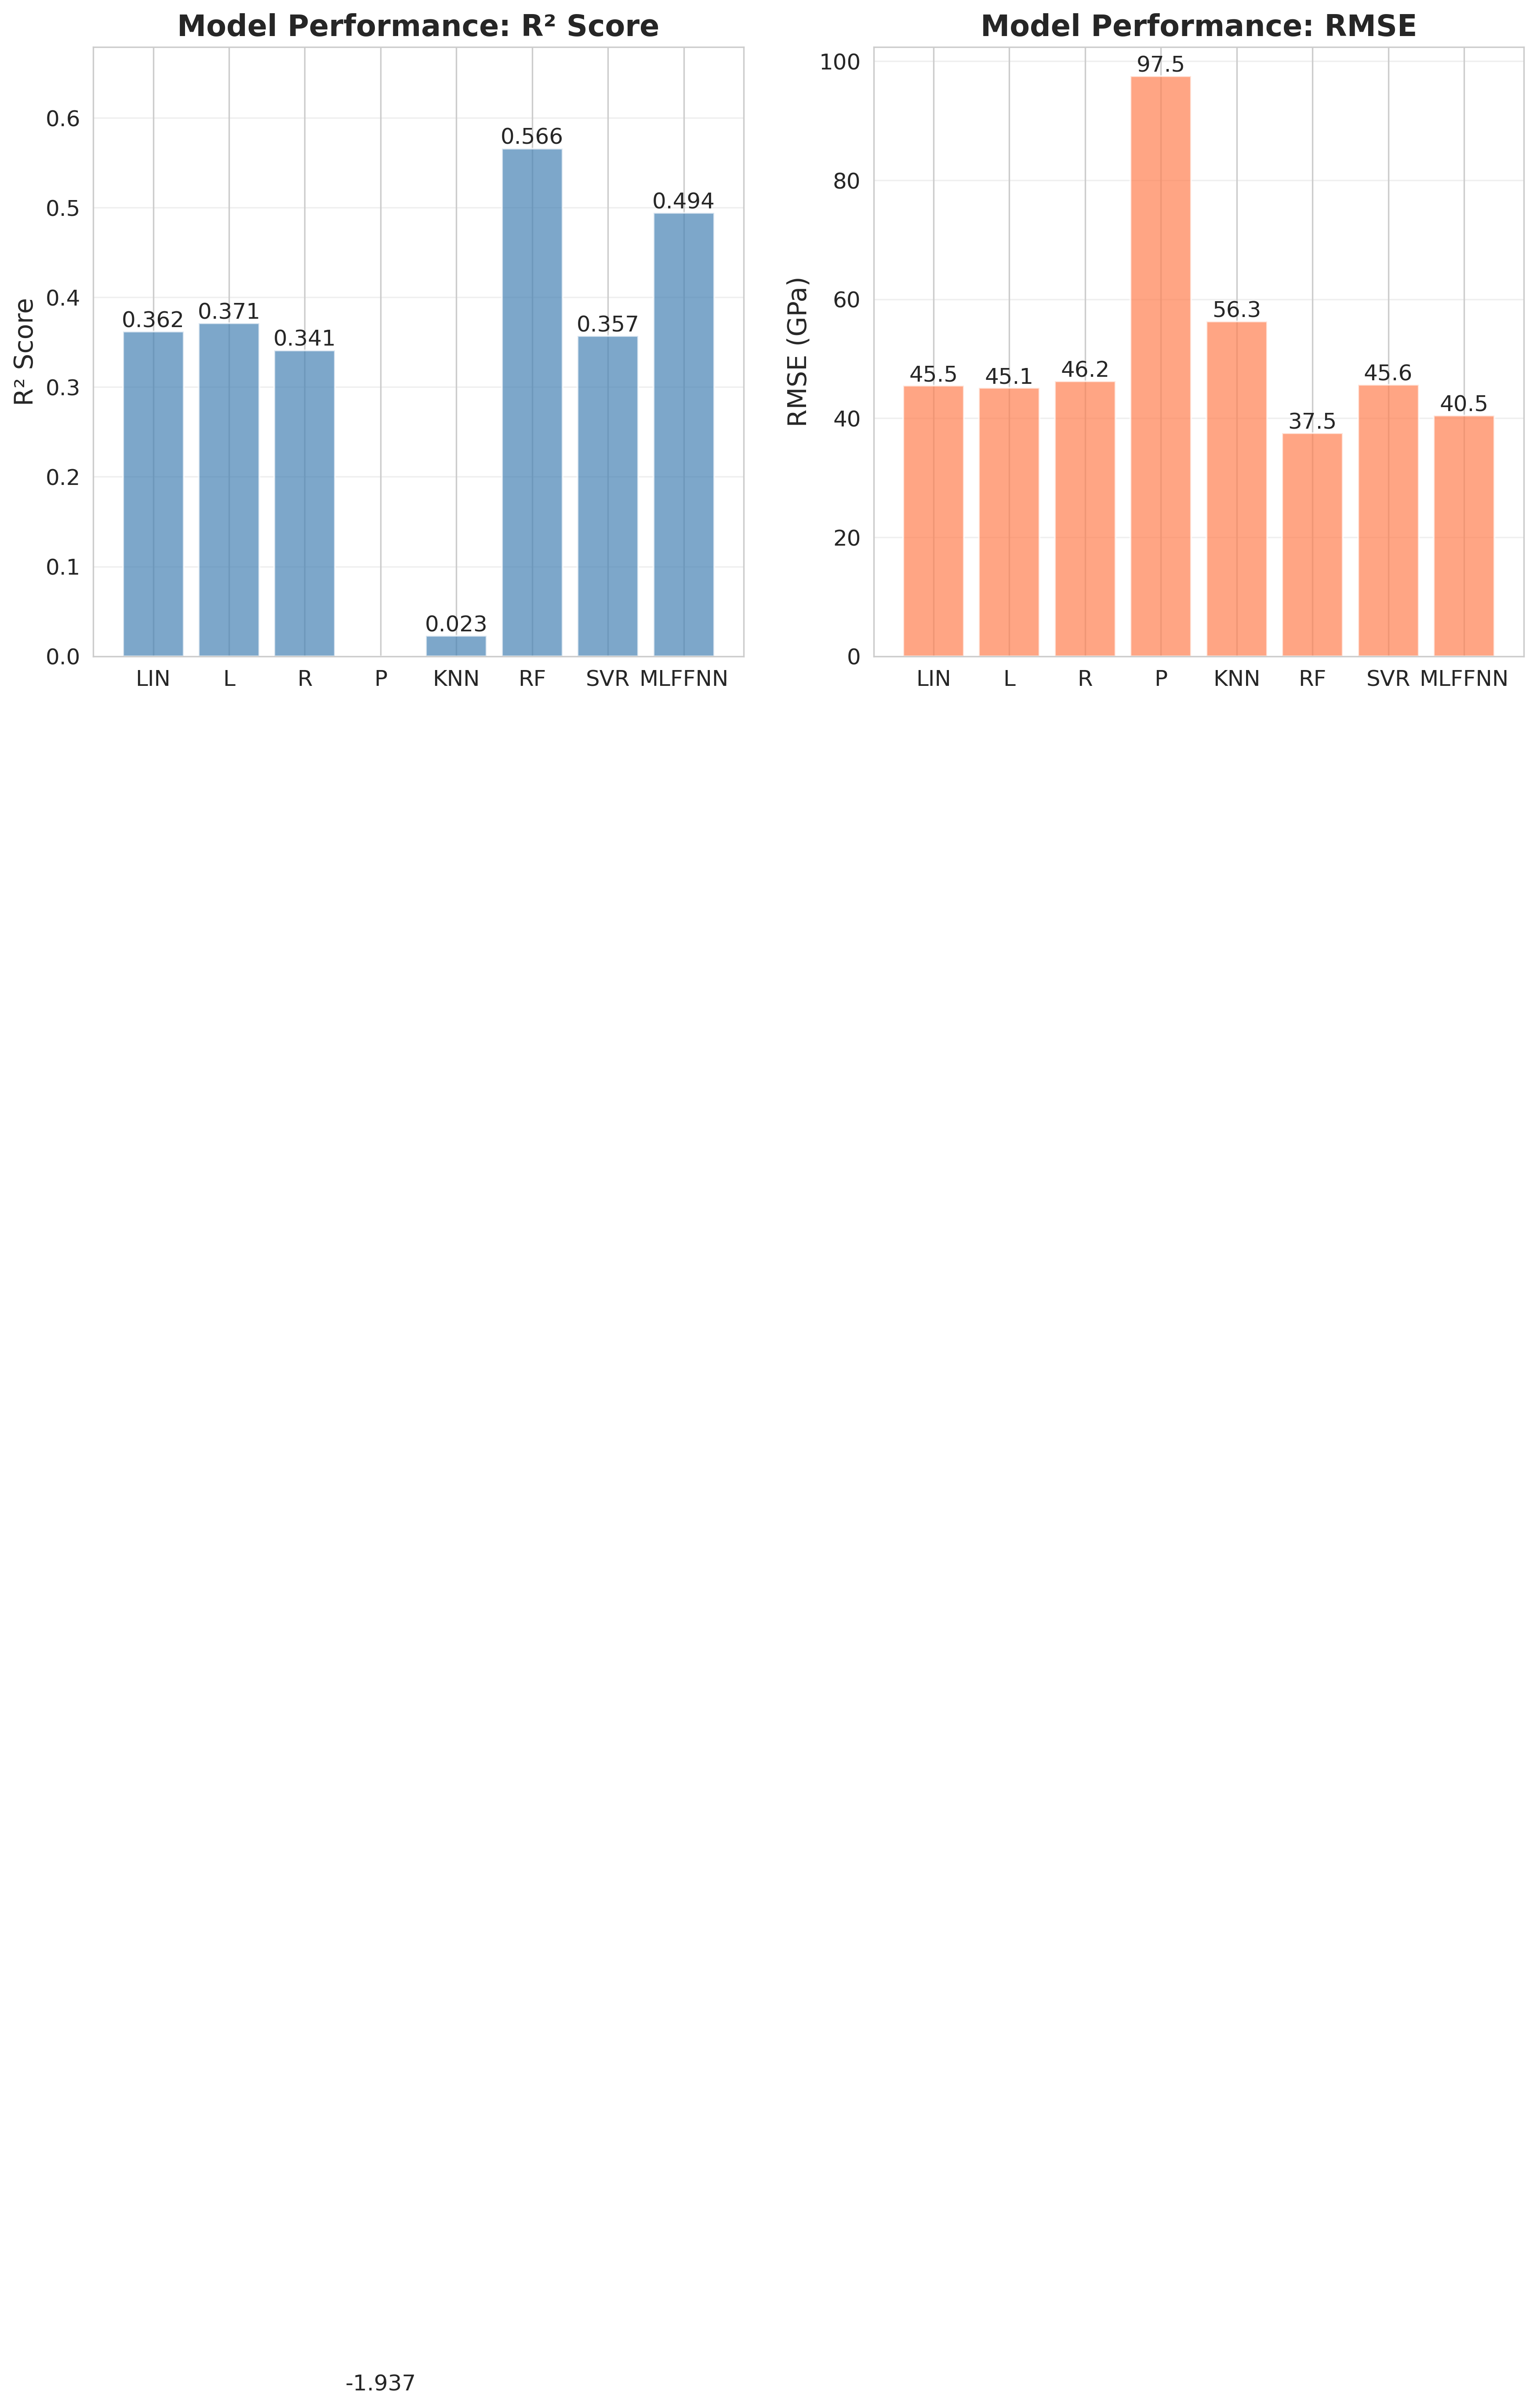
\includegraphics[width=0.85\textwidth]{figures/model_performance_comparison.png}
\caption{Comparison of model performance metrics (R$^2$ and RMSE) across different machine-learning algorithms. The optimized SVR and Gradient Boosting models show the best performance, with R$^2$ values of approximately 0.59 and 0.67, respectively.}
\label{fig:model_performance}
\end{figure}

\begin{figure}[htbp]
\centering
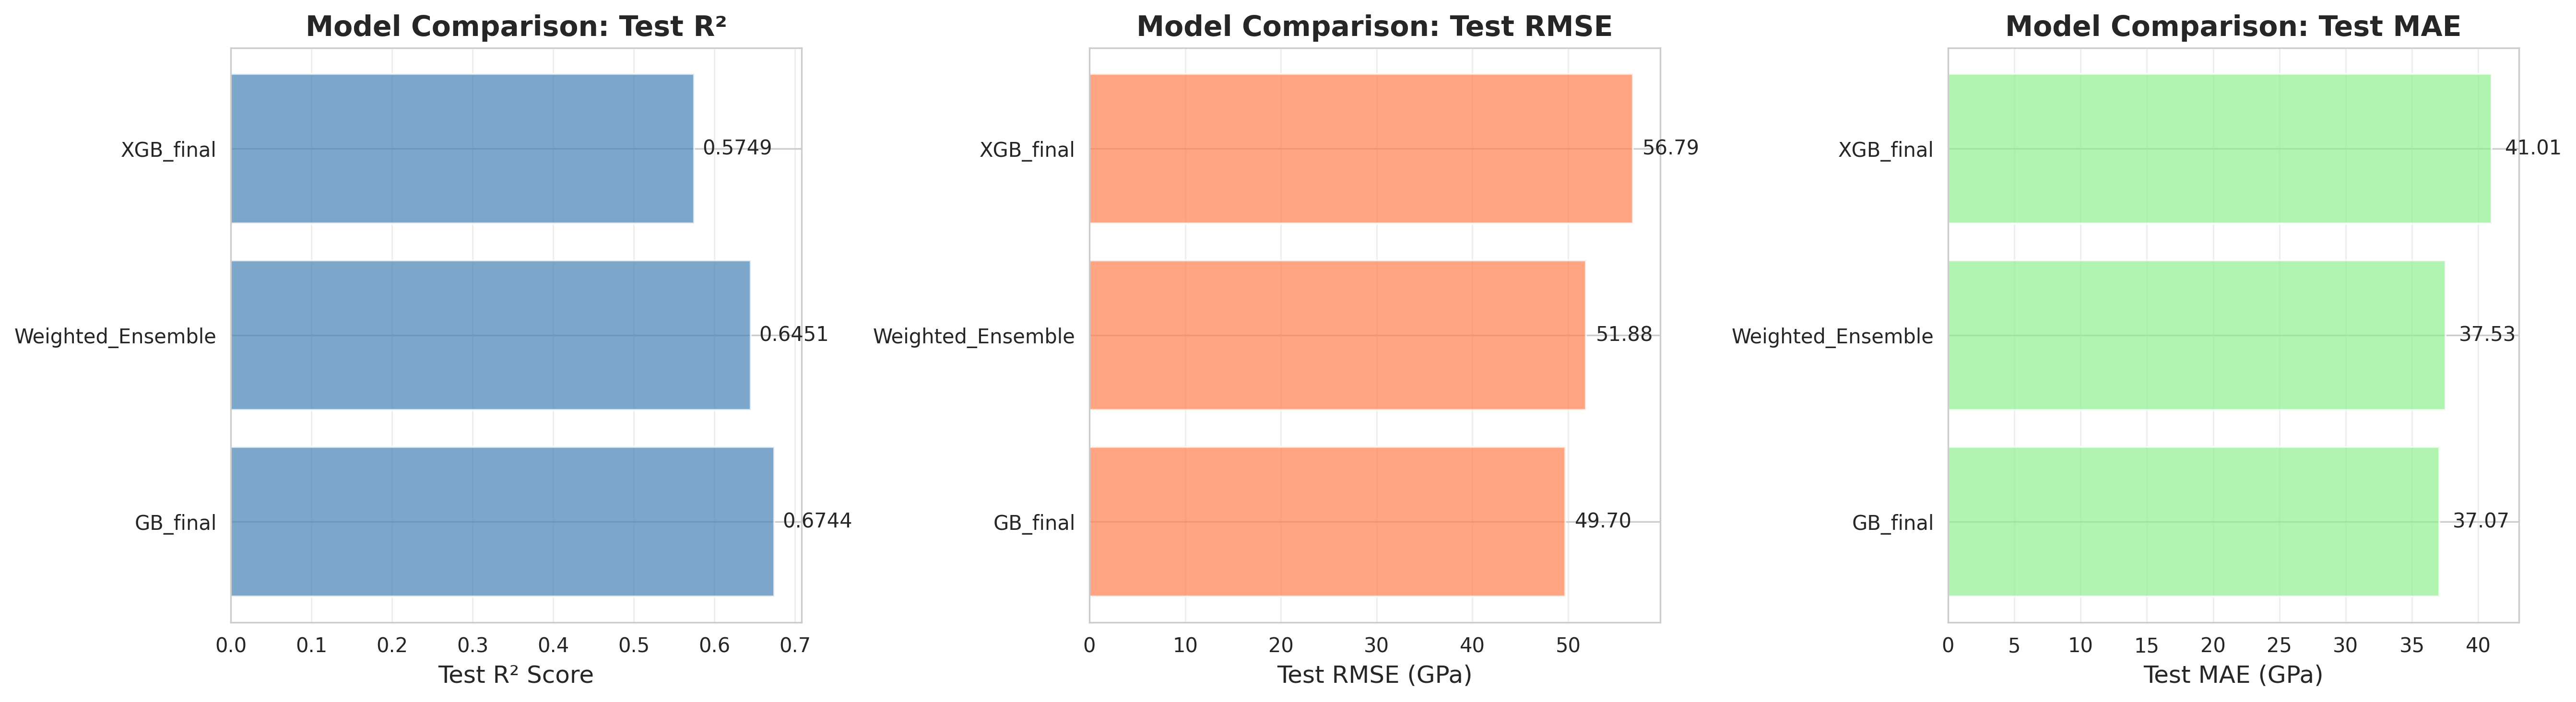
\includegraphics[width=0.85\textwidth]{figures/model_comparison_all.png}
\caption{Comprehensive comparison of all models showing performance across different metrics and data subsets. This visualization helps identify the best-performing models for different use cases.}
\label{fig:model_comparison_all}
\end{figure}

\begin{figure}[htbp]
\centering
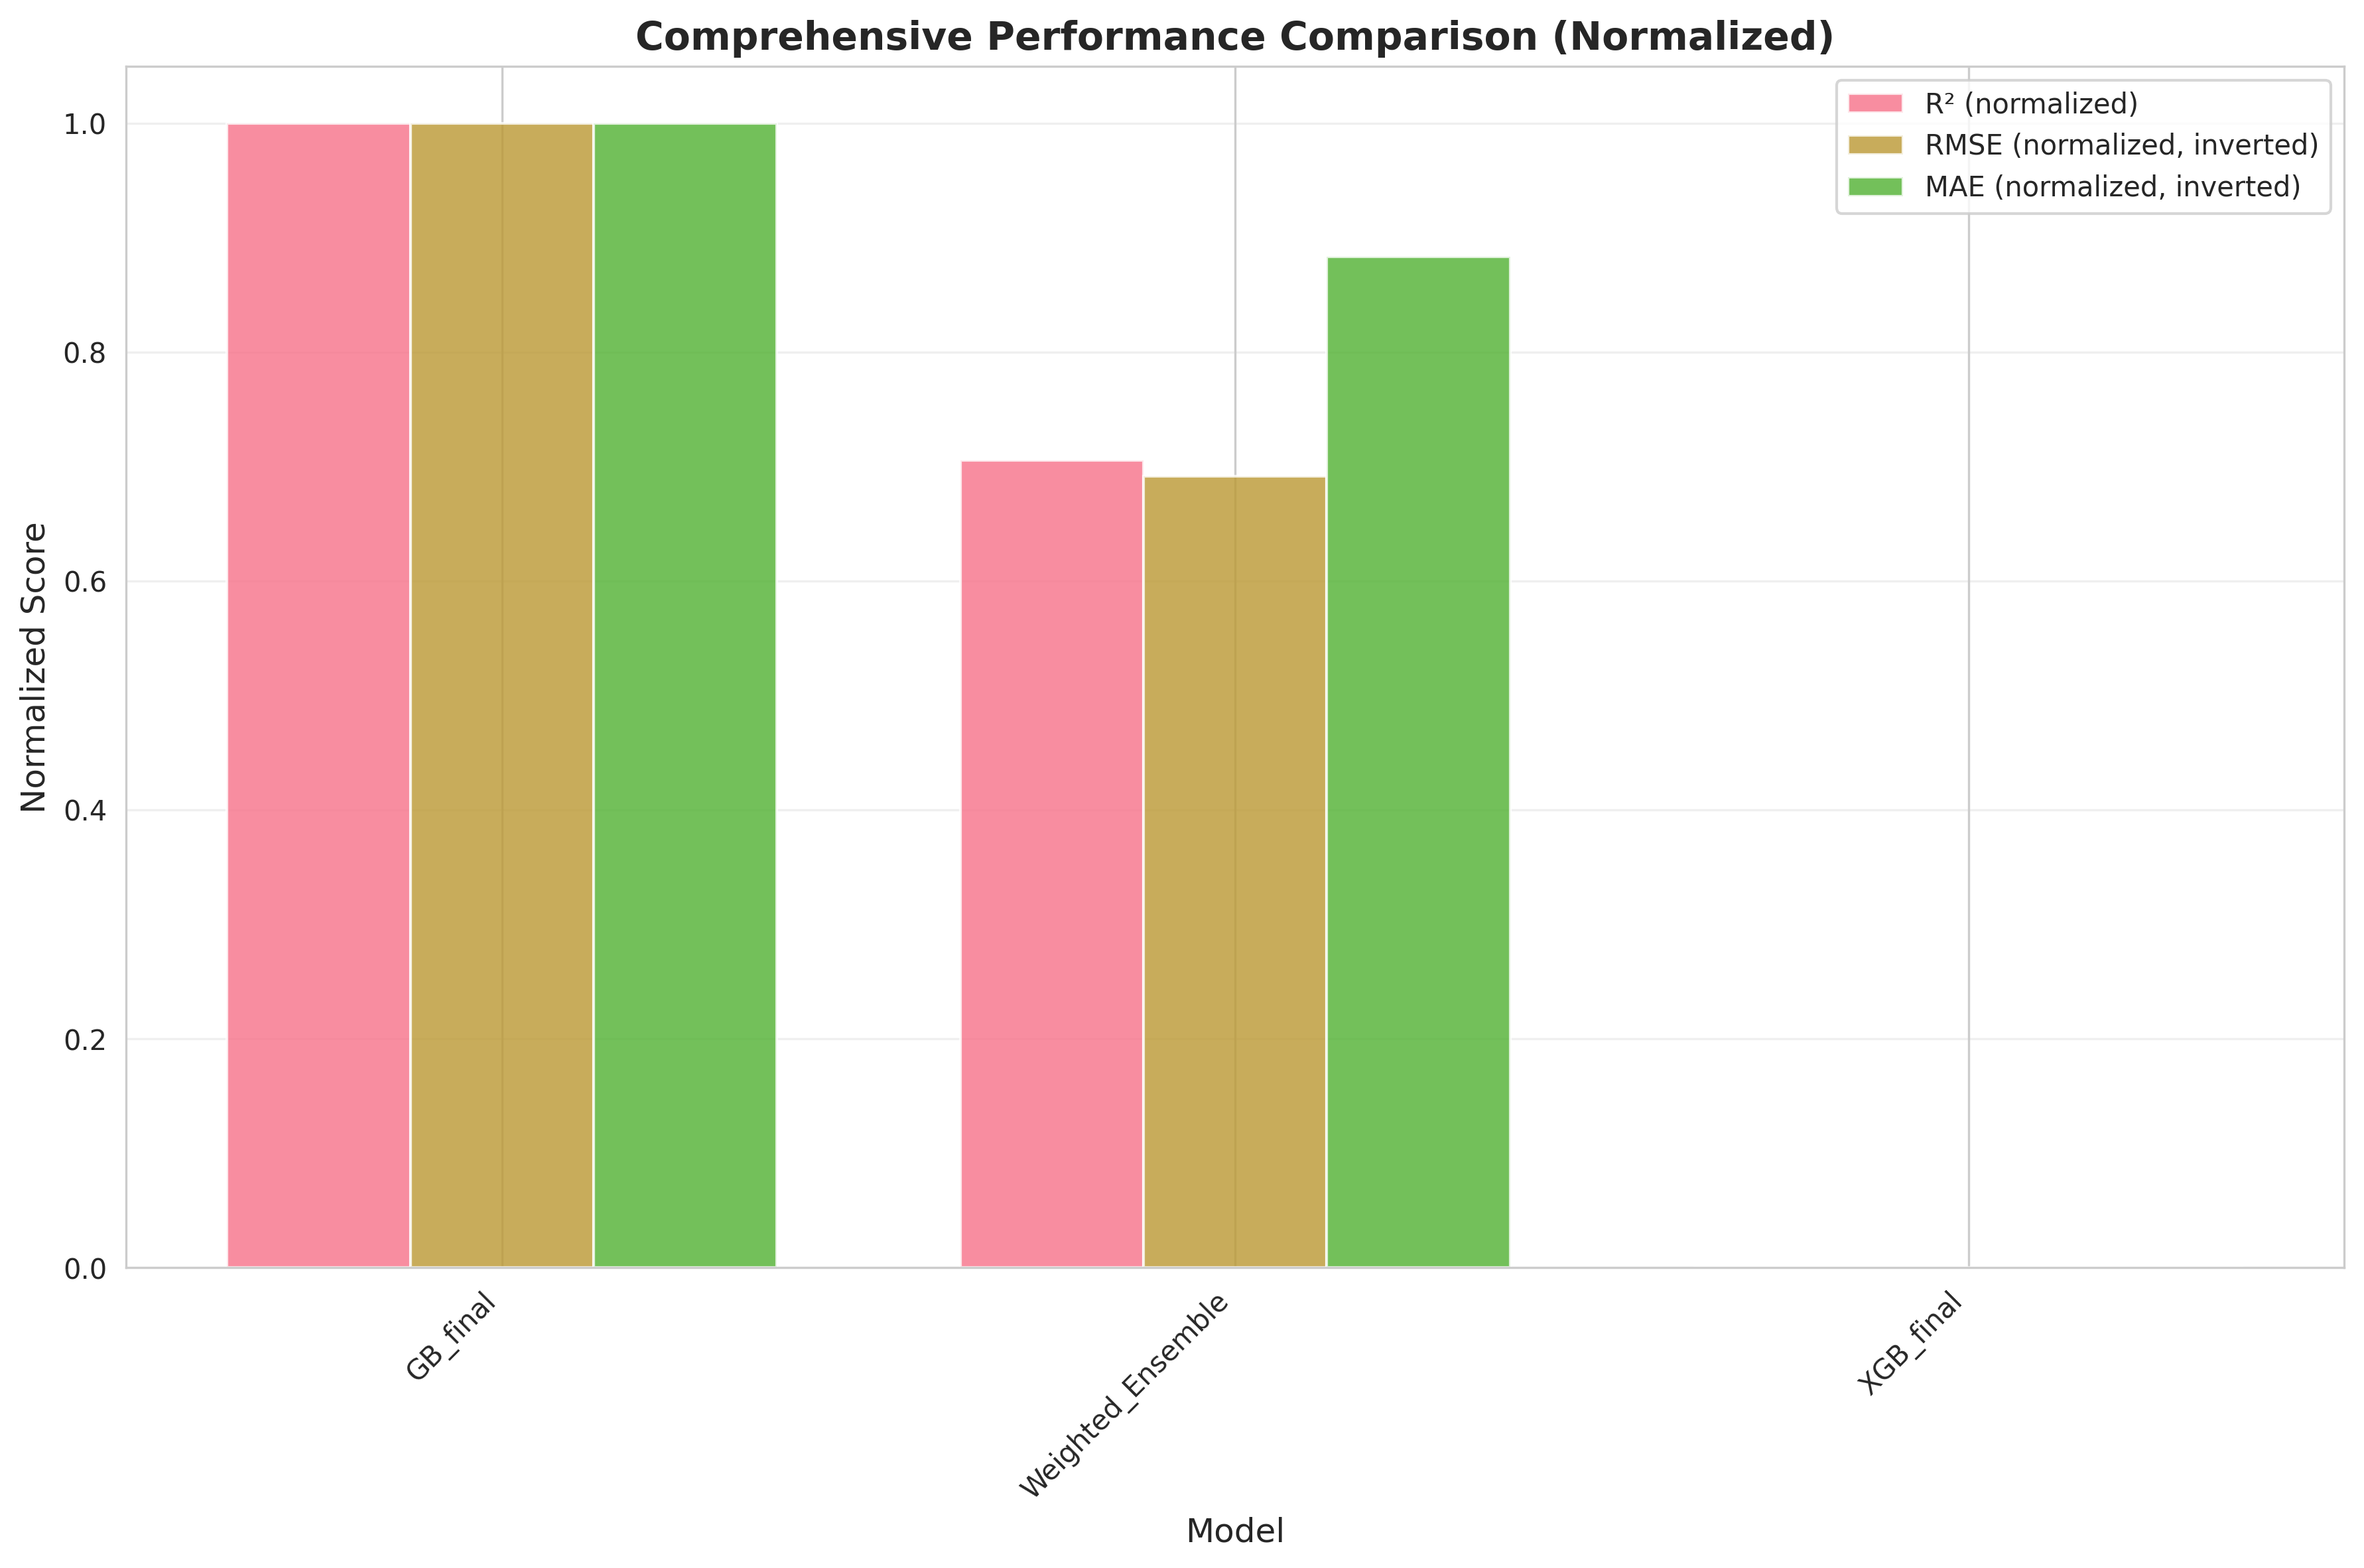
\includegraphics[width=0.85\textwidth]{figures/performance_metrics_comparison.png}
\caption{Detailed comparison of performance metrics (R$^2$, RMSE, MAE) for all evaluated models, highlighting the trade-offs between different evaluation criteria.}
\label{fig:performance_metrics}
\end{figure}

\subsection{Cross-Validation Results}

We also ran 5-fold cross-validation on the 322-sample dataset. Gradient Boosting gives a mean CV $R^2 = 0.48 \pm 0.09$, noticeably lower than its single-split test $R^2 = 0.67$ on the experimental-only subset. This gap is not surprising given the small sample size: each fold contains only $\sim$65 test points, so individual splits can vary considerably. A stacking ensemble (Gradient Boosting + SVR) yields a similar CV $R^2 \approx 0.48$ (test $R^2 = 0.48$, RMSE = 41.1~GPa, MAE = 26.3~GPa), so stacking does not help much at this data scale.

Feature-importance analyses from random forest and gradient boosting consistently identify the Ti composition fraction, average electronegativity, VEC, Co composition fraction, and density as dominant contributors. These trends support intuitive design guidelines for tuning elastic modulus, such as leveraging Ti-rich, lower-density compositions to reduce stiffness while carefully balancing refractory elements that increase modulus.

\begin{figure}[htbp]
\centering
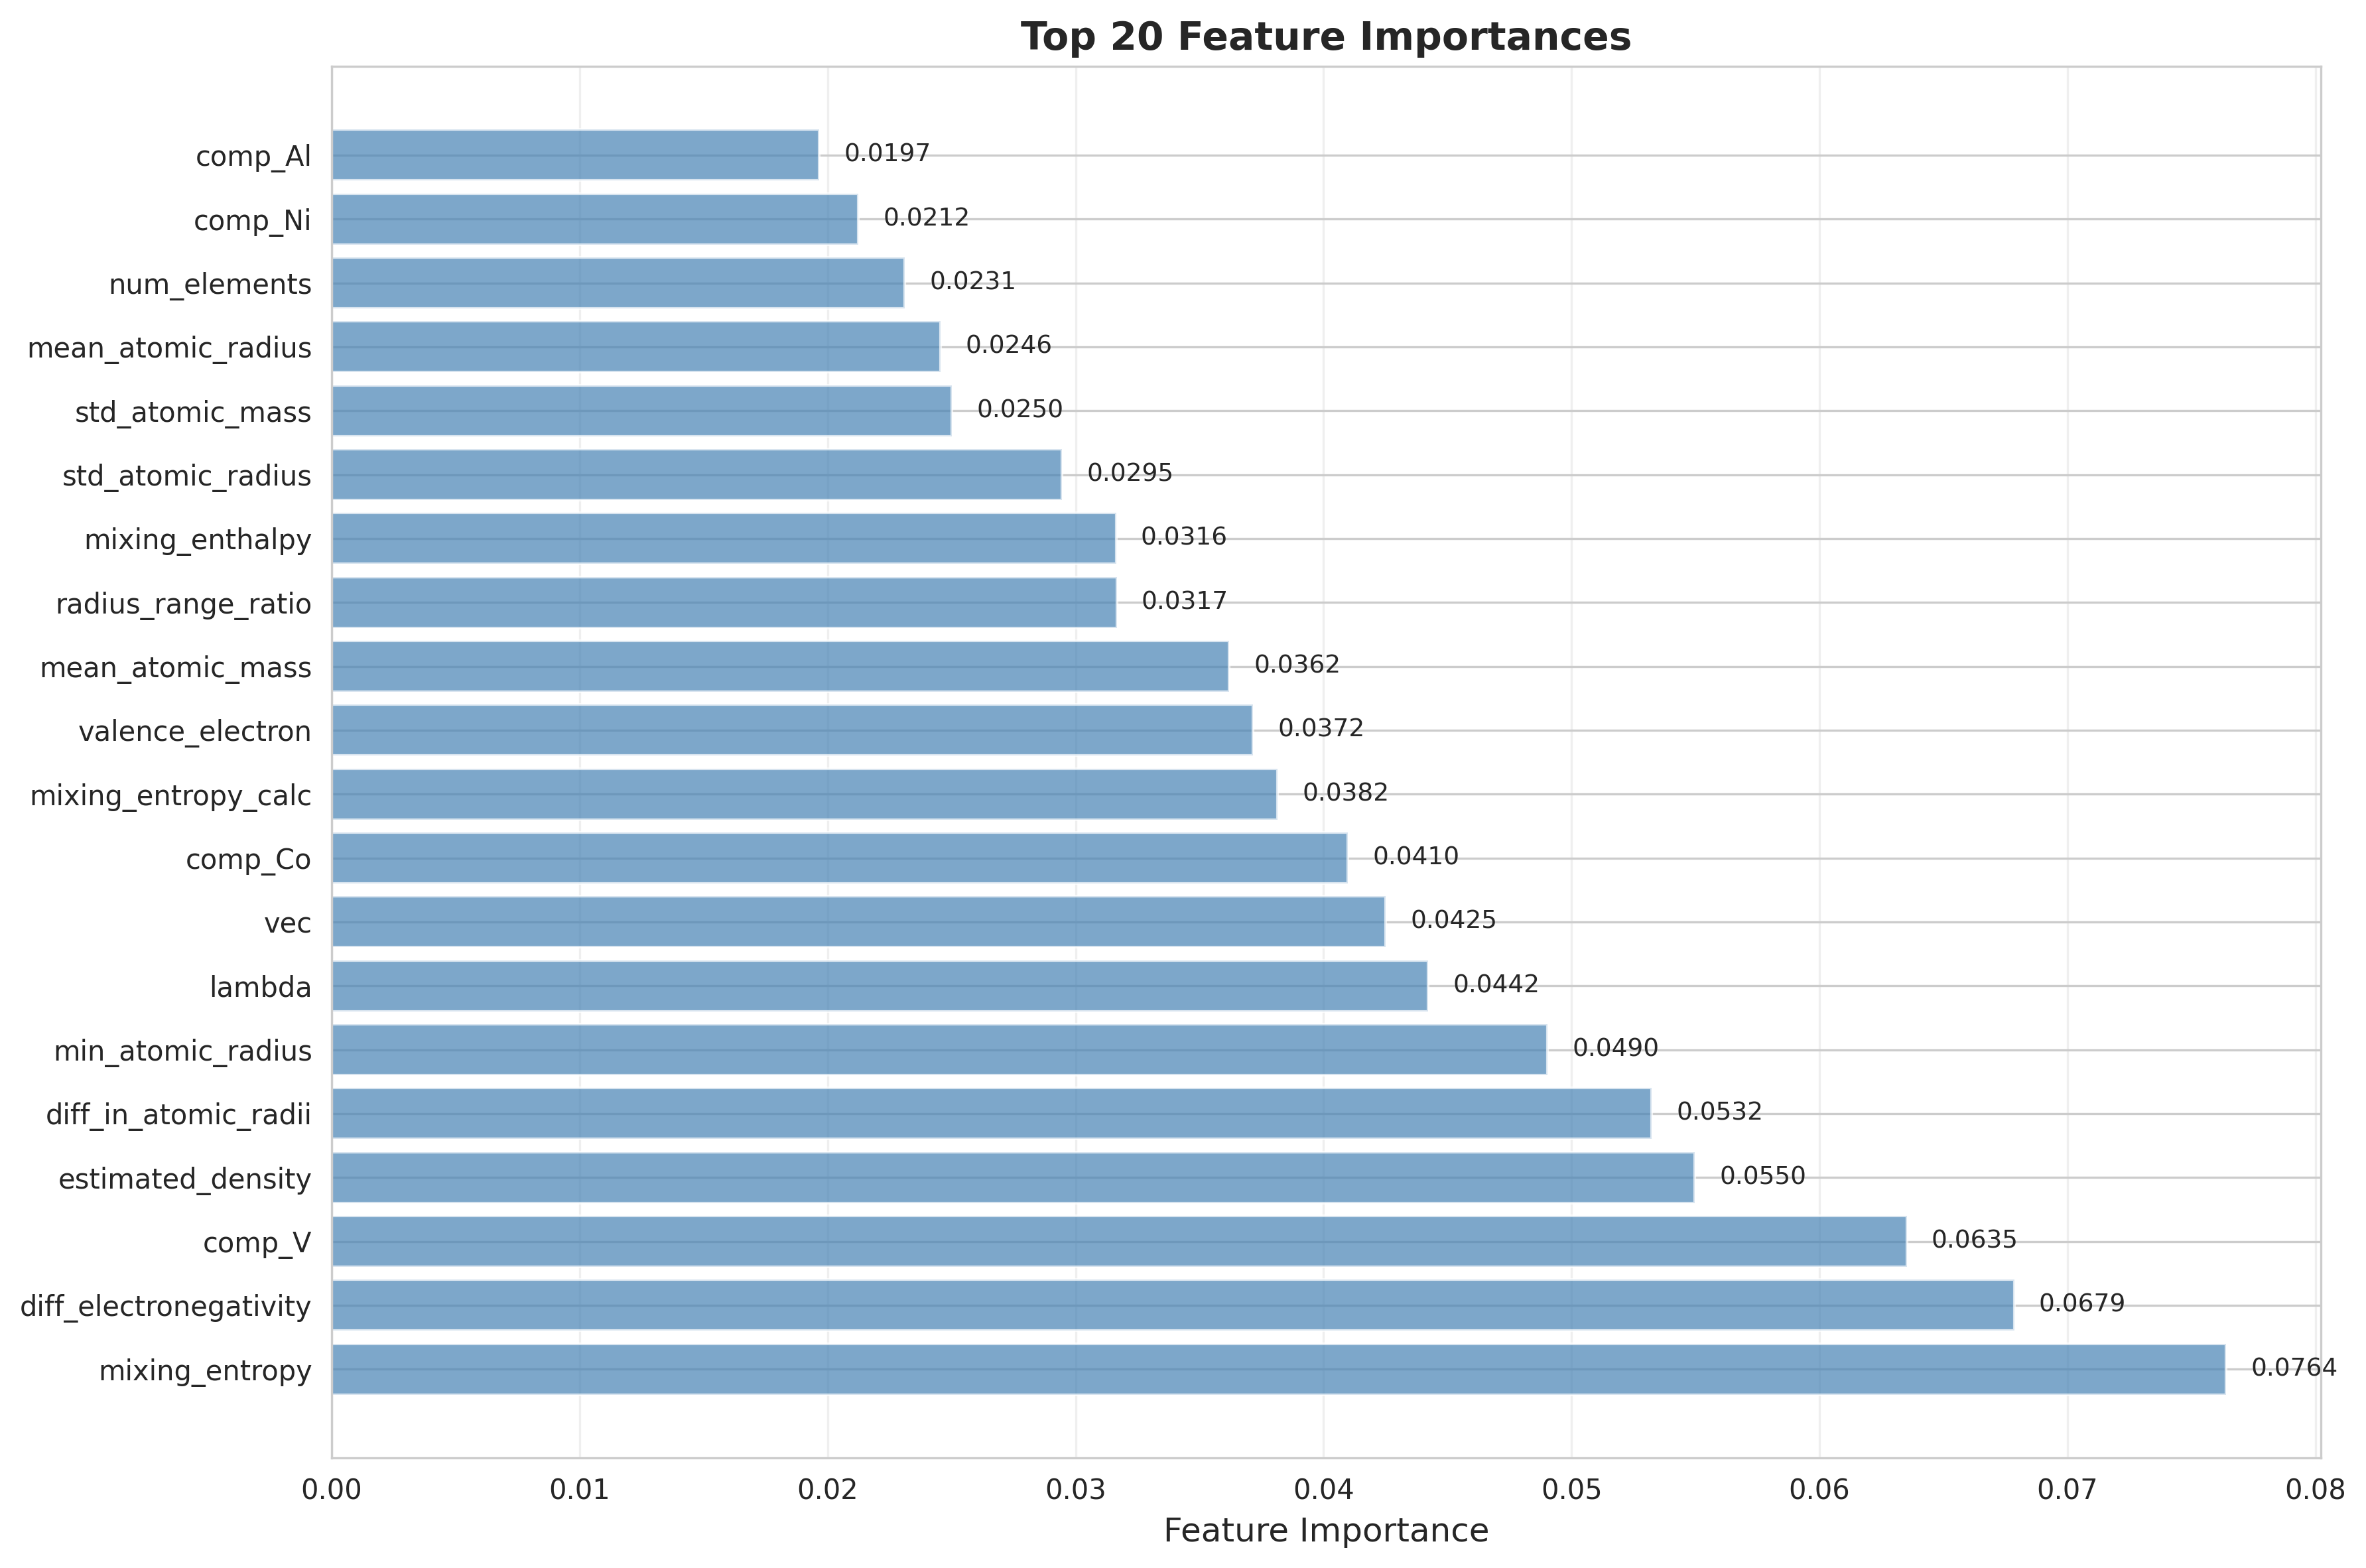
\includegraphics[width=0.85\textwidth]{figures/feature_importance.png}
\caption{Feature importance analysis from Random Forest regression. The Ti composition fraction (\texttt{comp\_Ti}) shows the highest importance (approximately 16--17\%), followed by average electronegativity, valence electron concentration (VEC), Co composition fraction, and density.}
\label{fig:feature_importance}
\end{figure}

\begin{figure}[htbp]
\centering
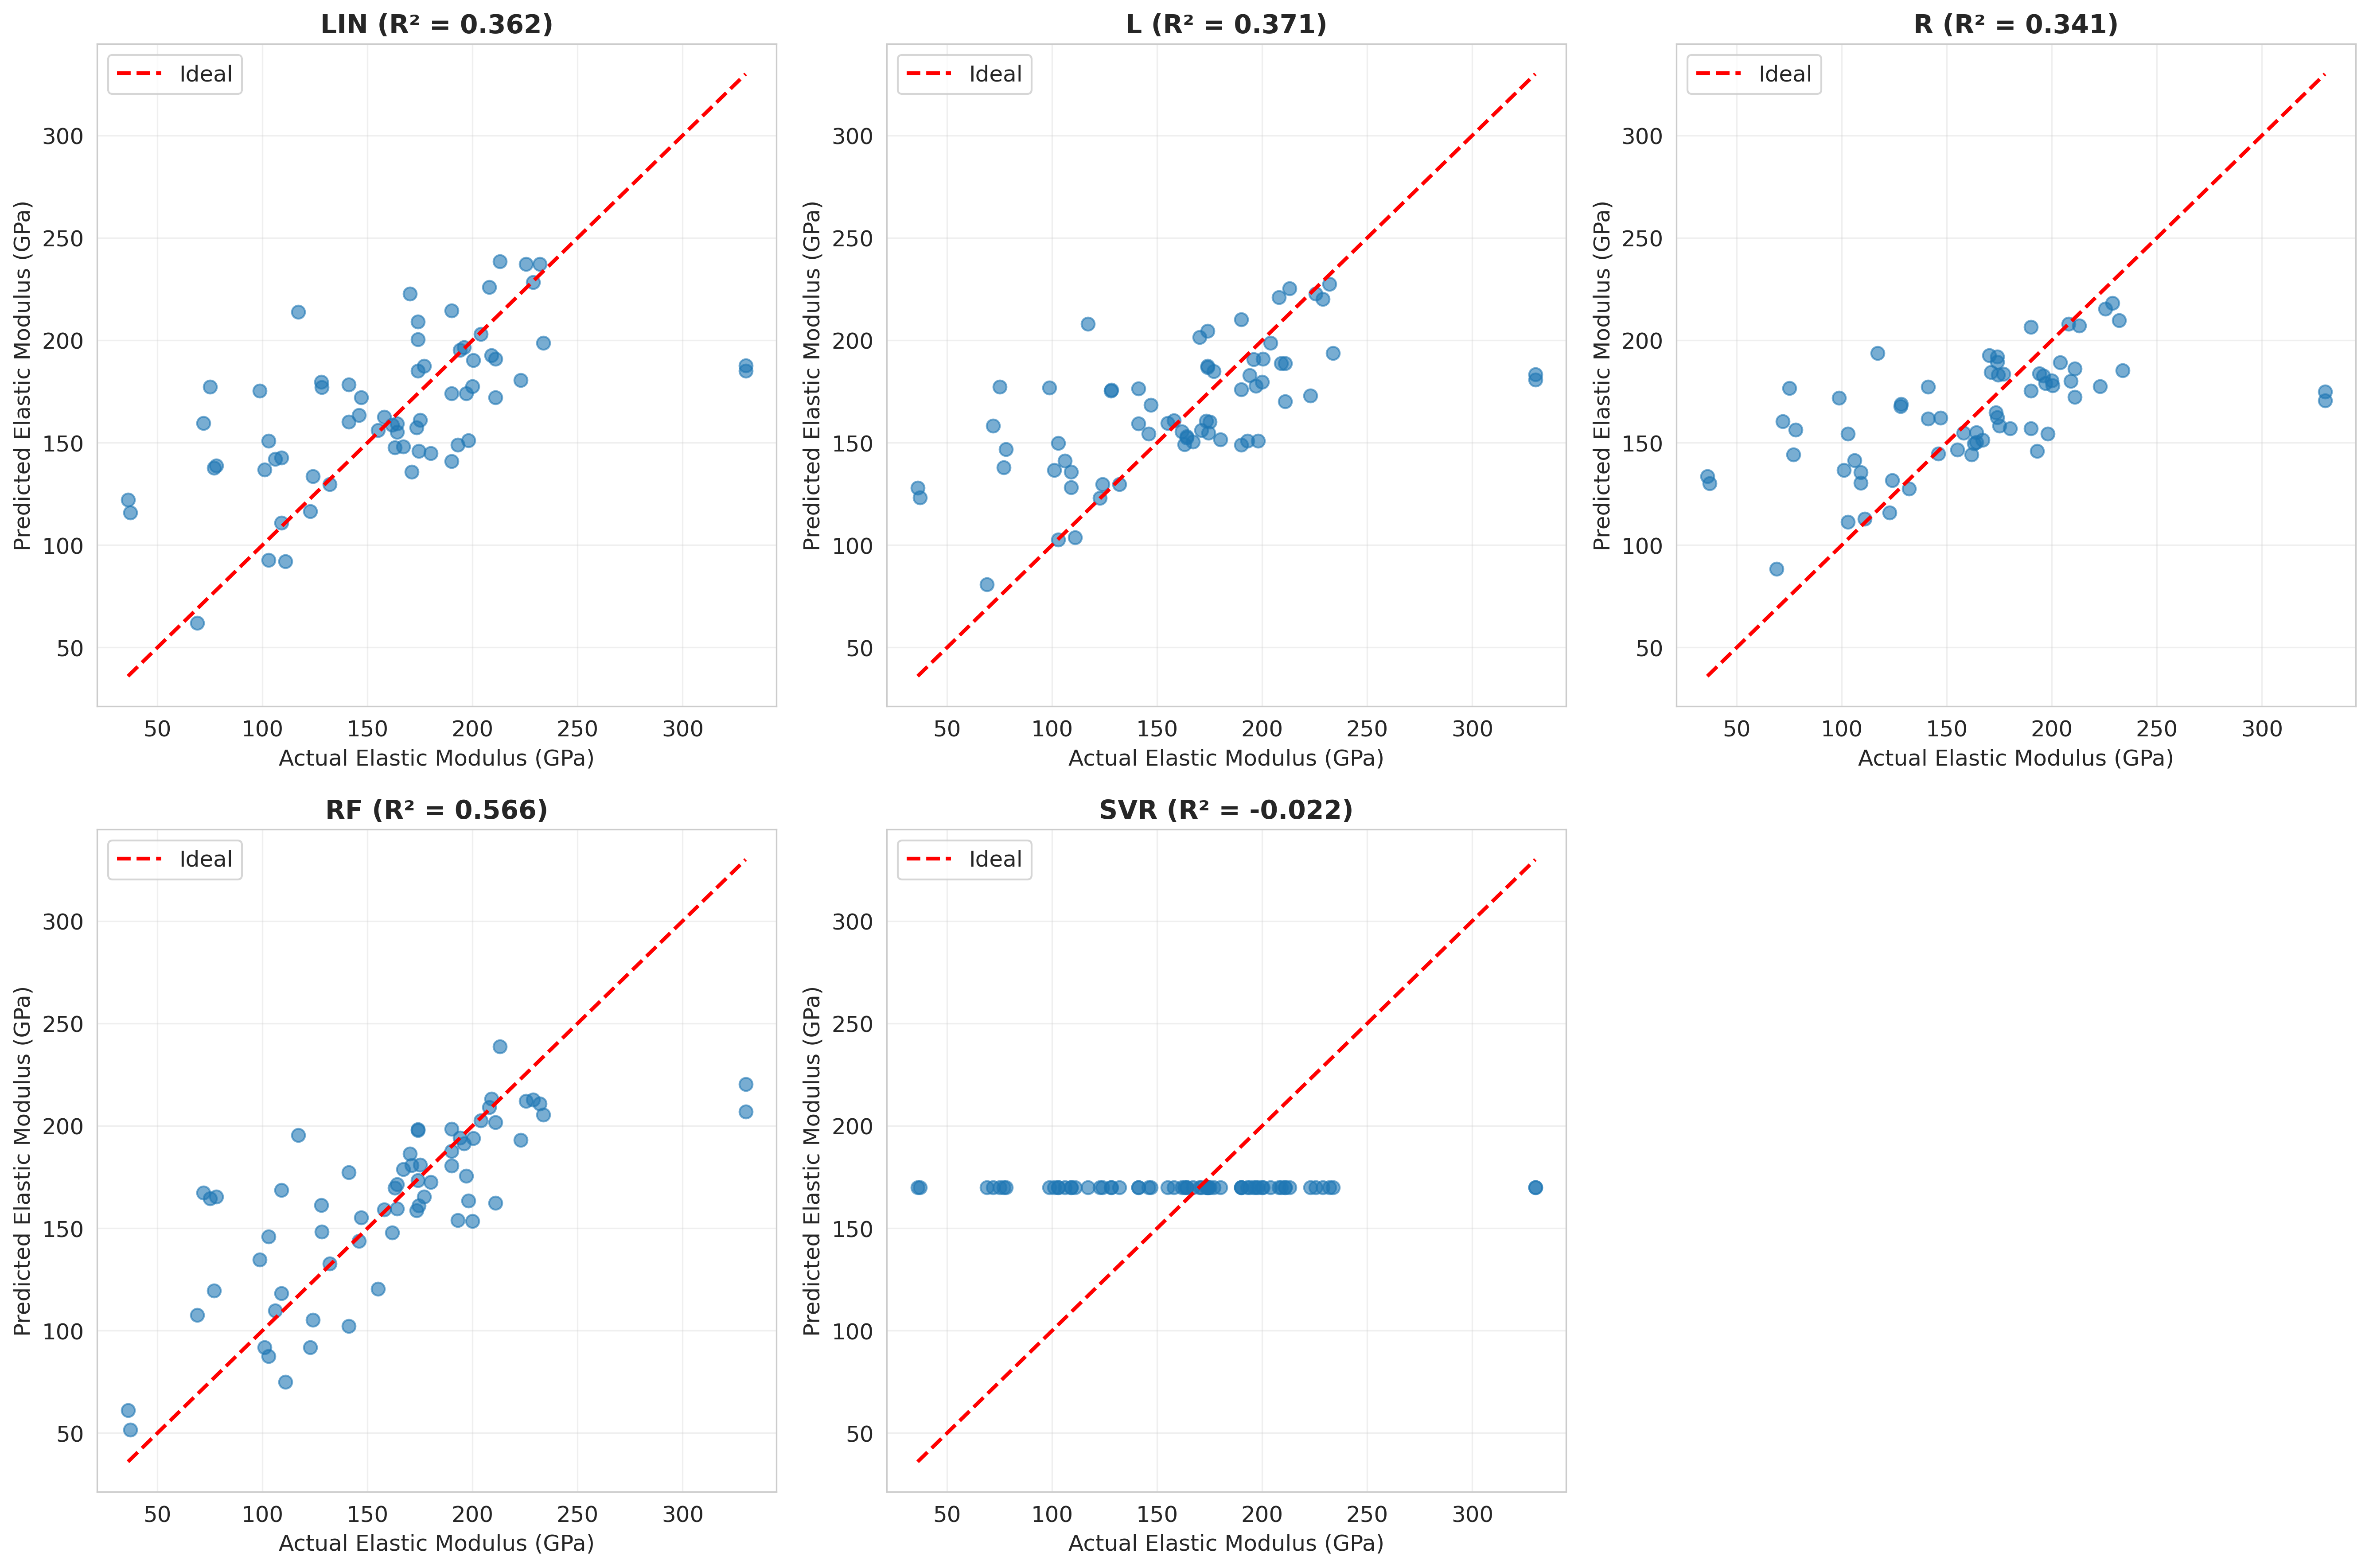
\includegraphics[width=0.85\textwidth]{figures/predicted_vs_actual.png}
\caption{Predicted vs.\ actual elastic modulus values for selected models on the 322-sample dataset. Random Forest ($R^2=0.57$) shows the best performance among baseline models. The diagonal line represents perfect prediction. Note: the SVR subplot shows baseline (unoptimized) performance ($R^2=-0.02$); the optimized SVR achieves $R^2=0.59$ after hyperparameter tuning.}
\label{fig:predicted_vs_actual}
\end{figure}

\begin{figure}[htbp]
\centering
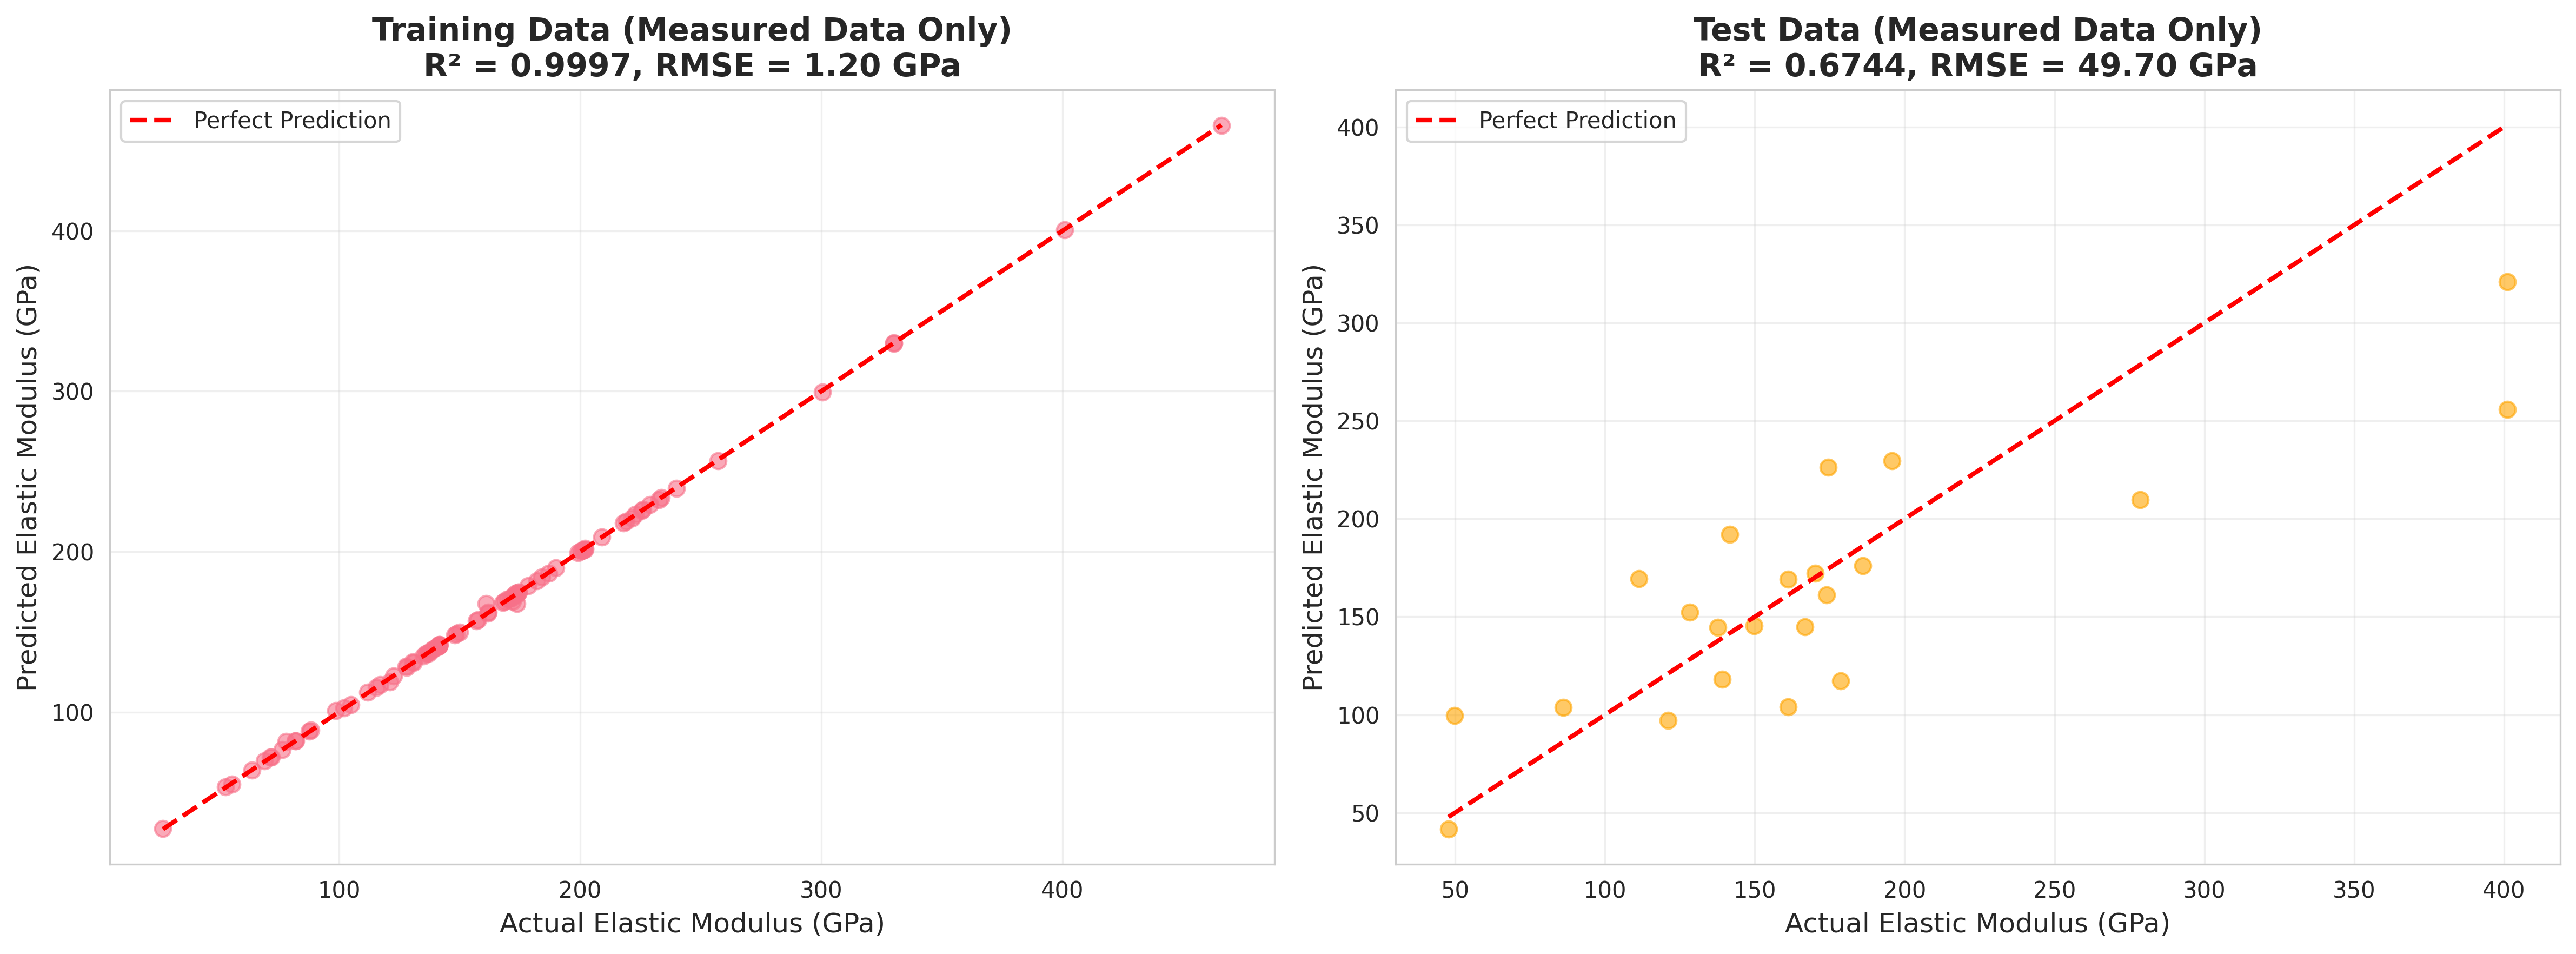
\includegraphics[width=0.85\textwidth]{figures/predicted_vs_actual_(measured_data_only).png}
\caption{Predicted vs.\ actual elastic modulus for models evaluated on the experimental-only subset. This comparison helps assess model performance when applied to purely experimental data, avoiding potential biases from computed values.}
\label{fig:predicted_vs_actual_measured}
\end{figure}

\begin{figure}[htbp]
\centering
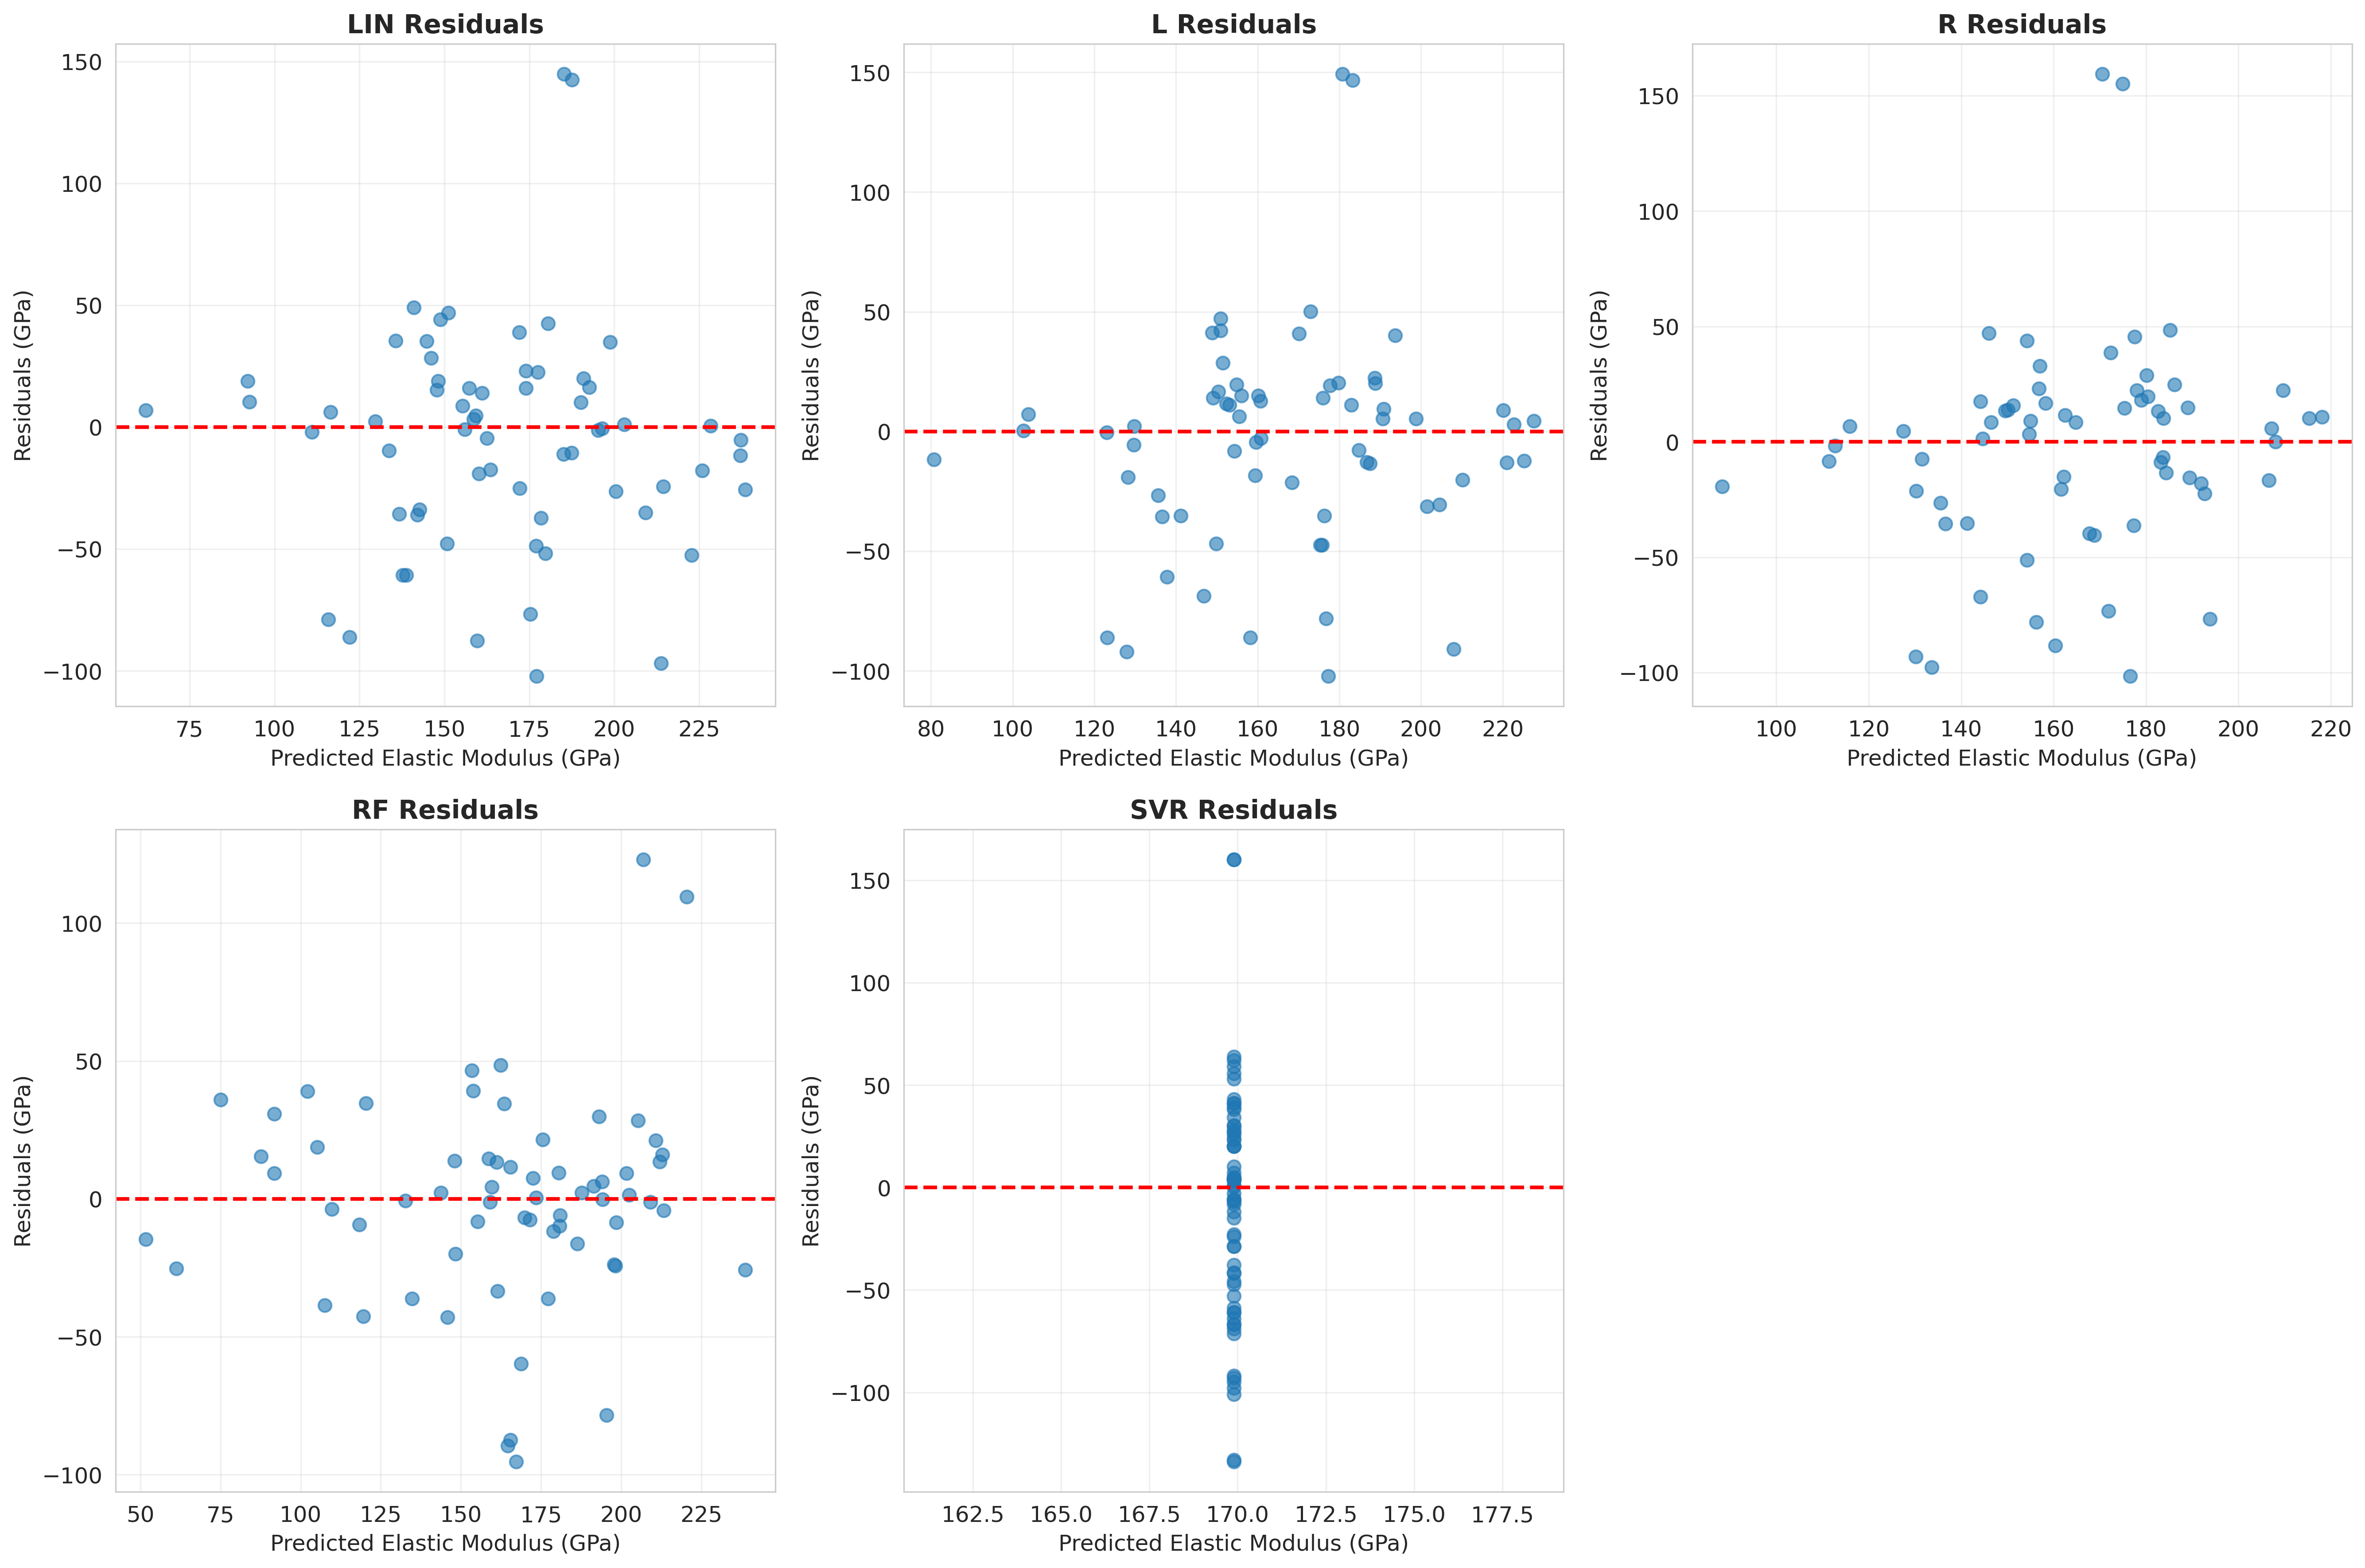
\includegraphics[width=0.85\textwidth]{figures/residuals_analysis.png}
\caption{Residual analysis for the optimized SVR model. The residuals are approximately centered around zero with no strong systematic trends, suggesting that the model captures the main relationships without severe bias. Larger errors tend to occur at the extremes of the modulus distribution.}
\label{fig:residuals}
\end{figure}

\begin{figure}[htbp]
\centering
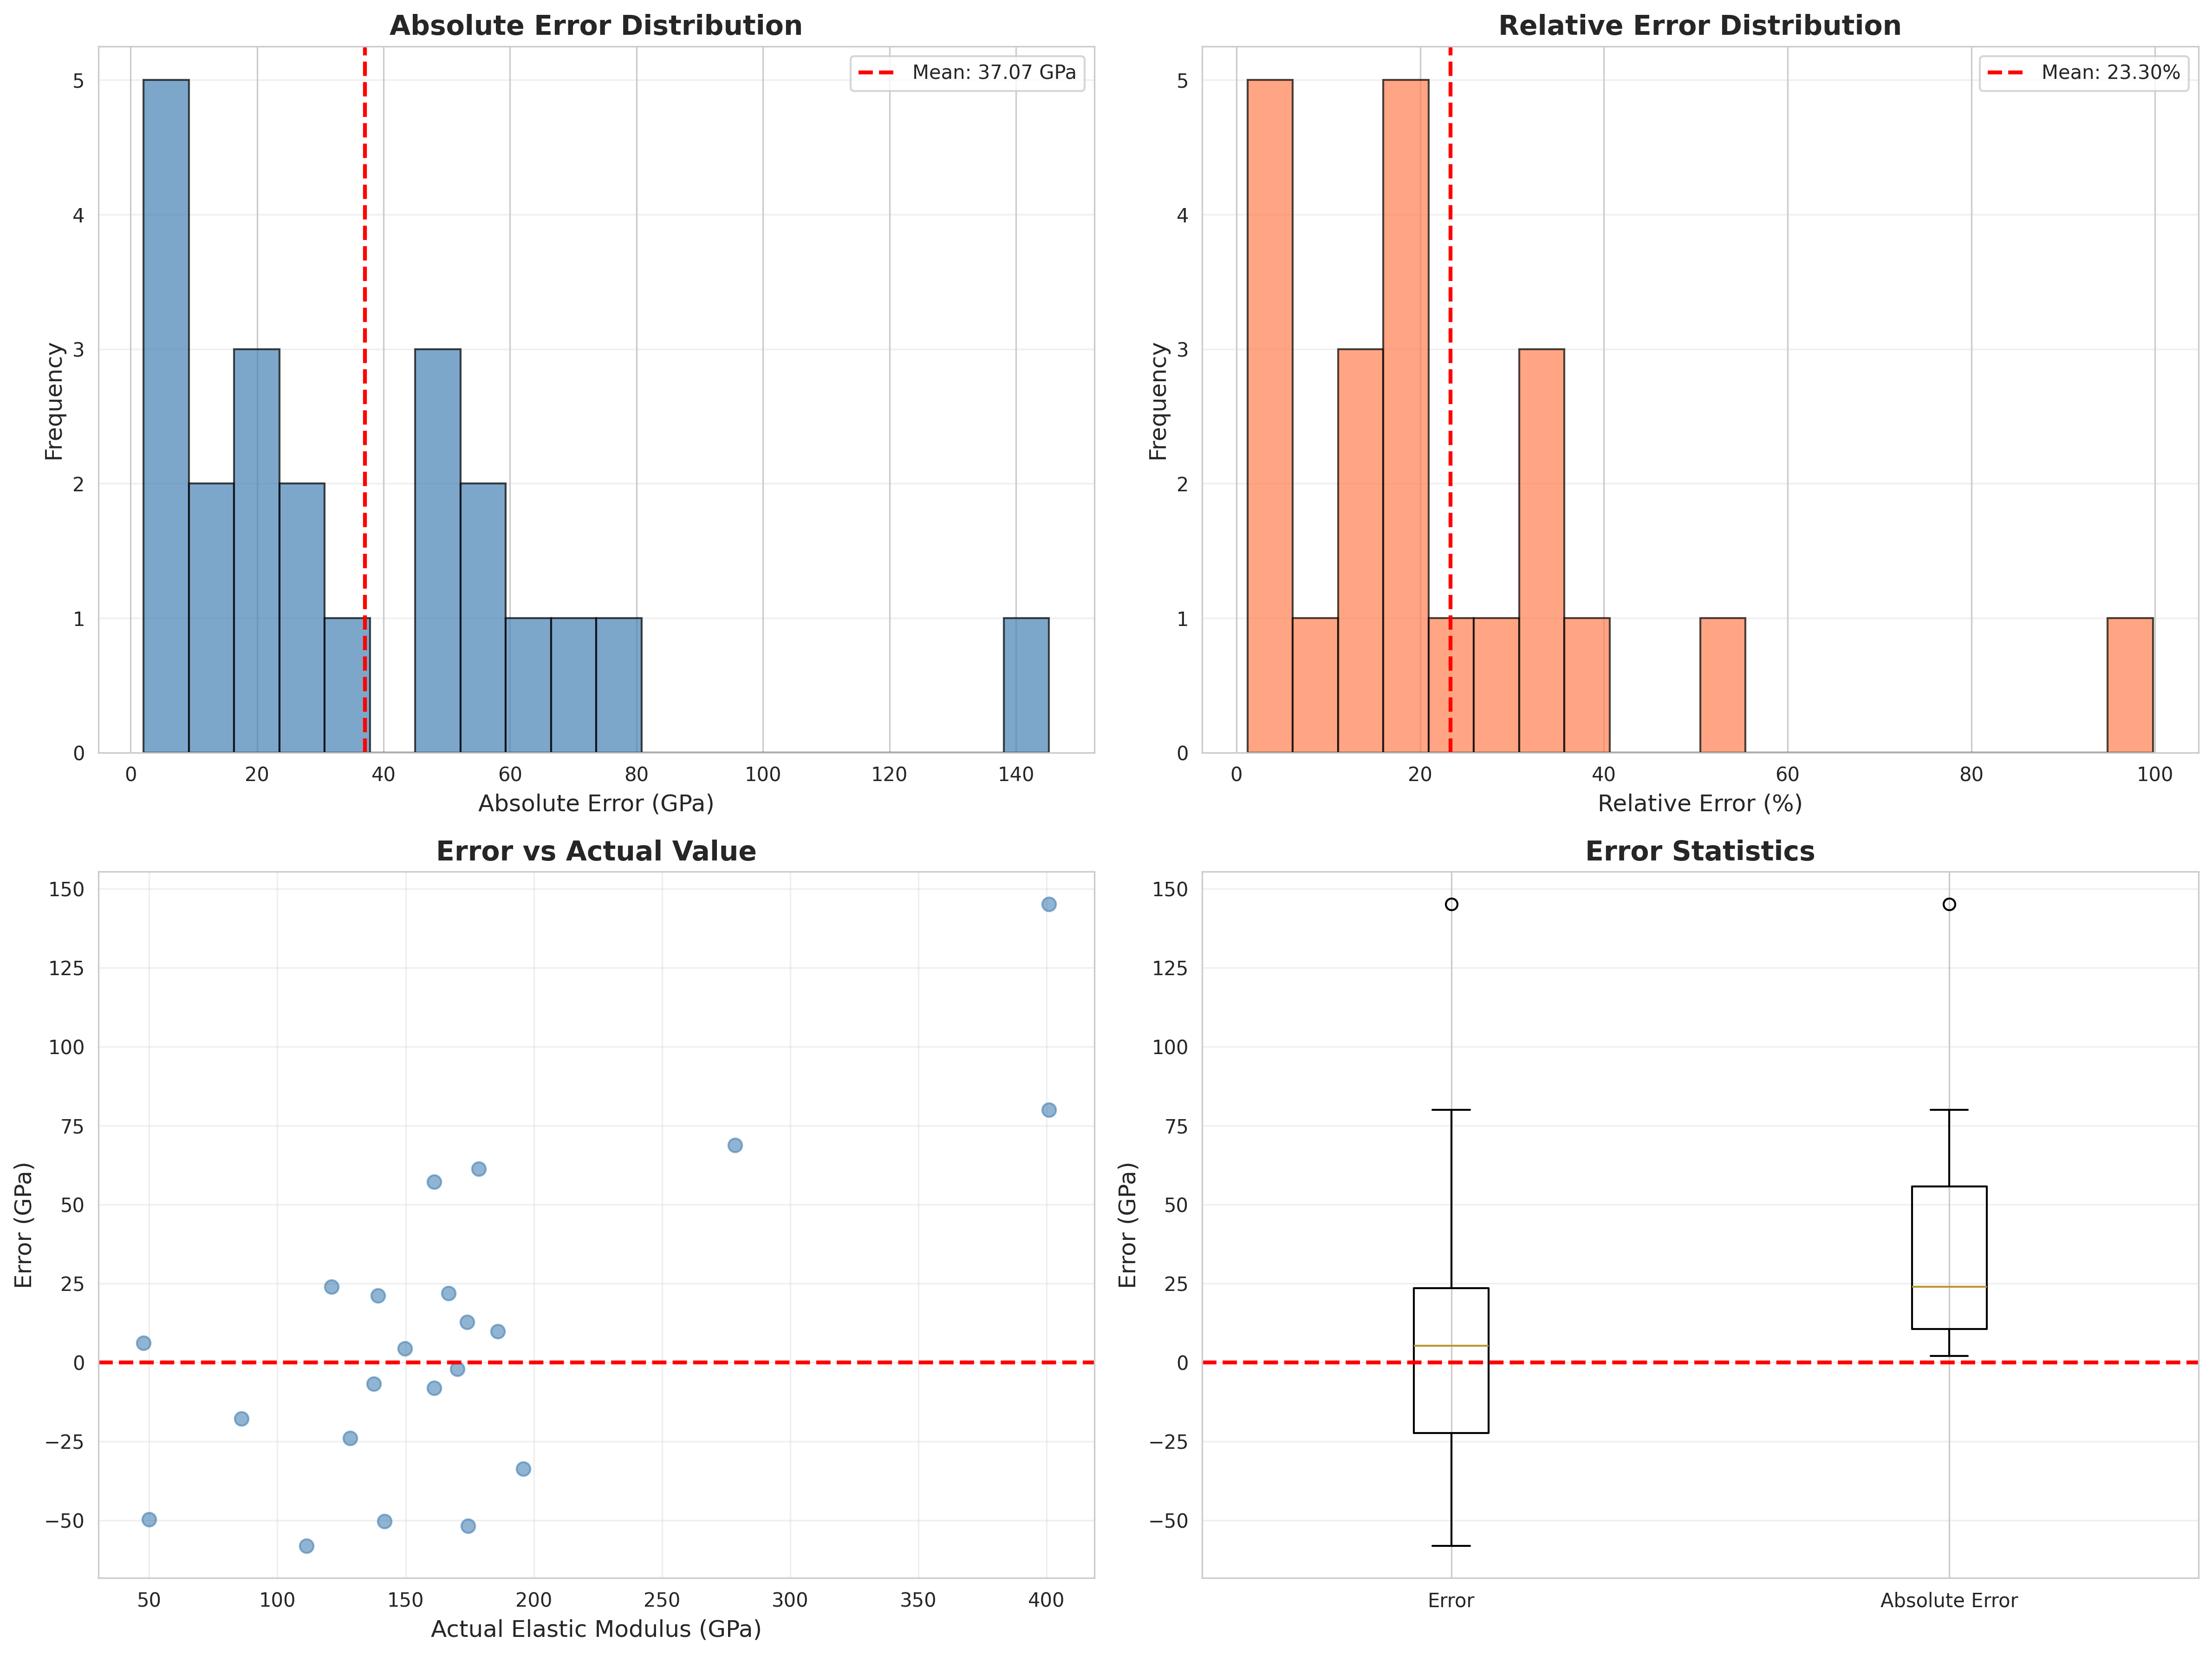
\includegraphics[width=0.85\textwidth]{figures/error_distribution.png}
\caption{Distribution of prediction errors across all models. The error distributions help identify systematic biases and assess the reliability of predictions for different modulus ranges.}
\label{fig:error_distribution}
\end{figure}

\begin{figure}[htbp]
\centering
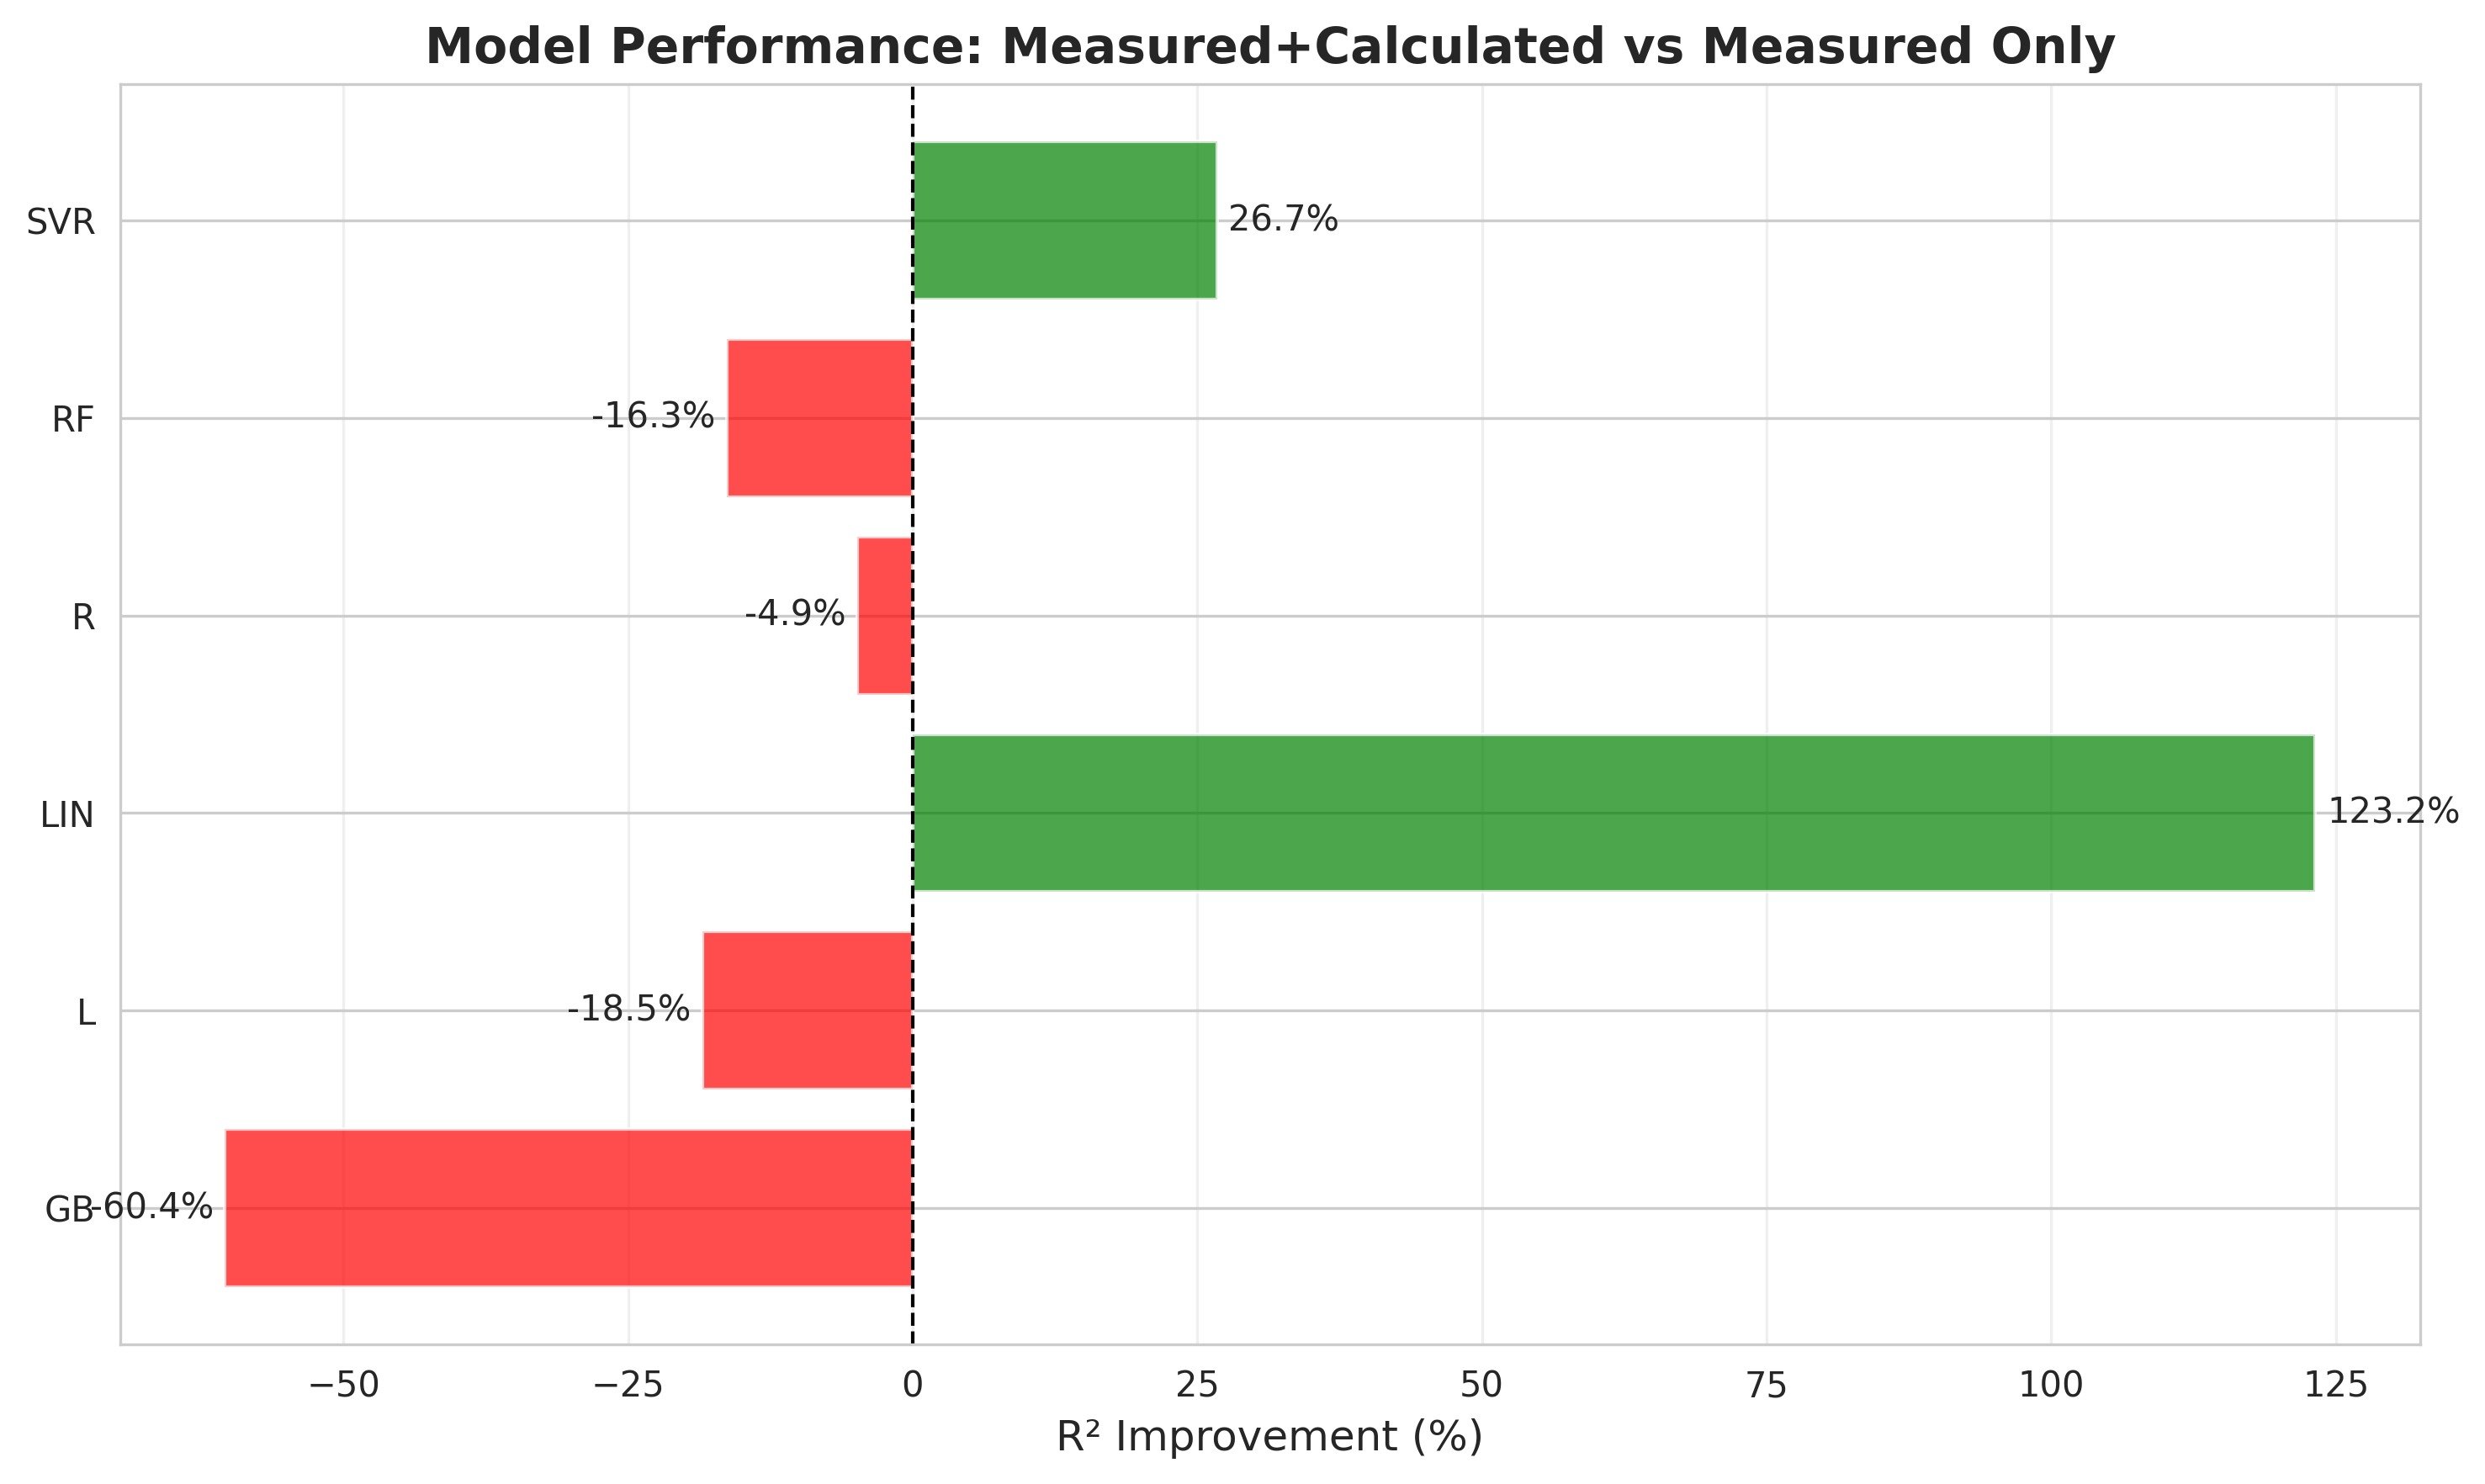
\includegraphics[width=0.85\textwidth]{figures/performance_improvement.png}
\caption{Performance improvement achieved through hyperparameter optimization. The comparison shows the gains from systematic tuning of model parameters, particularly for SVR and Gradient Boosting models.}
\label{fig:performance_improvement}
\end{figure}

The integrated dataset mixes experimental and computed data. While this greatly expands coverage of composition space, it also introduces systematic differences (e.g., DFT overestimation of modulus, lack of temperature and processing information). We therefore recommend training models on the full dataset but placing particular emphasis on evaluation and interpretation on experimental-only subsets.

\subsection{Comprehensive Model Evaluation on Full Dataset}

Table~\ref{tab:comprehensive_results} collects the results for all model families---classical ML, graph neural networks, neural operators, and the Transformer---evaluated on the full 5{,}339-sample dataset (deep-learning models) or the 322-sample subset (classical models).

\begin{table}[htbp]
\centering
\caption{Comprehensive model performance comparison. Classical ML models were evaluated on the 322-sample experimental subset, while deep-learning models (GNN, neural operators, Transformer) were evaluated on the full 5{,}339-sample integrated dataset. Performance metrics include coefficient of determination ($R^2$), root mean squared error (RMSE), and mean absolute error (MAE). $^\dagger$Transformer result ($R^2=0.62$) represents the best result from hyperparameter search across multiple training sessions on the 322-sample dataset; other training configurations yielded $R^2$ values of $-0.24$ and $0.05$, confirming the sensitivity of attention-based models to initialization and hyperparameters.}
\label{tab:comprehensive_results}
\begin{tabular}{lccc}
\hline
\textbf{Model} & \textbf{Test $R^2$} & \textbf{Test RMSE (GPa)} & \textbf{Test MAE (GPa)} \\
\hline
\multicolumn{4}{l}{\textit{Classical Machine Learning Models}} \\
\hline
Gradient Boosting (exp.\ only) & 0.67 & 49.7 & 37.1 \\
SVR (optimized) & 0.59 & 36.2 & 24.8 \\
Random Forest & 0.57 & 37.5 & 25.9 \\
MLFFNN & 0.49 & 40.5 & 29.0 \\
\hline
\multicolumn{4}{l}{\textit{Graph Neural Networks}} \\
\hline
MEGNet & 0.485 & 63.79 & 43.59 \\
CGCNN & 0.451 & 65.88 & 44.50 \\
GNN (HEAGNN) & 0.259 & 49.08 & 29.53 \\
\hline
\multicolumn{4}{l}{\textit{Neural Operator and Physics-Informed Models}} \\
\hline
PINNs & 0.403 & 68.71 & 45.78 \\
Neural ODE & 0.254 & 76.77 & 53.46 \\
DeepONet & 0.275 & 75.68 & 53.08 \\
FNO & 0.243 & 77.33 & 53.46 \\
\hline
\multicolumn{4}{l}{\textit{Transformer-based Models}} \\
\hline
Transformer (HEATransformer)$^\dagger$ & 0.62 & 34.91 & 26.17 \\
\hline
\end{tabular}
\end{table}

\subsubsection{Key Findings}

Several patterns stand out from the results:

\begin{itemize}
  \item \textbf{Classical ML and Transformer lead}: Gradient Boosting ($R^2=0.67$), optimized SVR ($R^2=0.59$), and the HEATransformer ($R^2=0.62$, RMSE 34.9~GPa) all outperform the deep-learning alternatives. Well-tuned tree-based and kernel methods remain hard to beat at this dataset size.

  \item \textbf{Graph networks are moderate}: MEGNet ($R^2=0.485$) and CGCNN ($R^2=0.451$) learn useful representations but fall short of the classical models, likely because graph construction from composition alone (without crystal-structure input) limits the information available. HEAGNN ($R^2=0.259$) needs further architecture tuning.

  \item \textbf{Neural operators struggle}: FNO, DeepONet, and Neural ODE give $R^2$ in the range 0.24--0.28. These architectures assume spatially continuous input fields, which is a poor match for discrete alloy compositions. PINNs do somewhat better ($R^2=0.403$), perhaps because the physics loss provides additional regularization.
\end{itemize}

\subsubsection{Why Classical Models Win Here}

We attribute the performance ranking to three factors.  First, our 29 hand-crafted features already encode most of the relevant physics (atomic size, electronegativity, VEC); the classical models can exploit them directly, while graph and operator networks must re-learn equivalent representations from scratch.  Second, with only $\sim$5{,}300 samples the dataset is small by deep-learning standards, so highly parameterized models tend to overfit or underfit depending on initialization.  Third, the 94\% DFT / 6\% experimental split introduces a systematic bias---DFT overestimates elastic moduli---which may confuse models that lack explicit domain knowledge.

\subsubsection{Practical Recommendations}

For immediate use, SVR or Gradient Boosting with the 29-feature set offers the best trade-off between accuracy, speed, and interpretability.  For longer-term research, MEGNet and CGCNN are worth revisiting once larger experimental datasets become available.  A promising direction is to combine hand-crafted descriptors with attention or graph layers, so that domain knowledge and data-driven learning complement each other.

\subsection{Limitations}

The most obvious limitation is data imbalance: 94\% of the entries are DFT-computed, and DFT is known to systematically overestimate elastic moduli.  Models trained on the full dataset inevitably absorb this bias.  The experimental subset (322 samples, 109 for the experimental-only split) is small enough that single train/test splits can be misleading---the CV-vs-test gap for Gradient Boosting ($R^2_\text{CV}=0.48$ vs.\ $R^2_\text{test}=0.67$) makes this clear.

Beyond sample size, the dataset contains no information on processing temperature, heat treatment, or microstructure, all of which strongly affect stiffness in practice.  Coverage of composition space is also uneven: Ti--Zr--Nb systems and refractory HEAs are well represented, but predictions for alloy families outside this region should be taken with caution.

\section{Conclusion}

We assembled a 5{,}339-alloy dataset with elastic modulus labels and benchmarked models ranging from linear regression to graph neural networks and Transformers.  The main finding is that, at the current data scale, classical models with hand-crafted features (SVR: $R^2=0.59$; Gradient Boosting: $R^2=0.67$; HEATransformer: $R^2=0.62$) outperform more complex deep-learning architectures.  Graph networks reach $R^2 \approx 0.45$--$0.49$; neural operators stay below 0.28.

These results show that data-driven elastic-modulus prediction is feasible and can guide the search for low-modulus HEAs in the 30--90~GPa range relevant to bone implants.  At the same time, the dominance of classical methods signals that more experimental data and better input representations are needed before deep-learning approaches can justify their added complexity.

Next steps include growing the experimental portion of the dataset, adding uncertainty quantification, and exploring hybrid architectures that feed hand-crafted descriptors into graph or attention layers.

\section*{Acknowledgements and Data Availability}

The dataset and scripts used in this work are maintained in the AI\_metallurgy project repository under the \texttt{data\_collection} directory. Key source datasets include the Gorsse HEA mechanical-properties database, the DOE/OSTI high-entropy-alloy dataset, the Materials Project elastic-tensor database, and several MPEA and HEA mechanical-property compilations.

\subsection*{Final Dataset and Model Snapshots}

The following files represent the final, validated versions of the dataset and best-performing models:

\begin{itemize}
  \item \textbf{Final integrated dataset}: \texttt{final\_data/unified\_dataset\_latest.csv} (version: 2026-01-23, 5{,}339 samples)
  \item \textbf{Optimized SVR model} (best performance on full 322-sample dataset): \texttt{models/model\_SVR\_optimized.pkl} with \texttt{scaler\_SVR\_optimized.pkl}
  \item \textbf{Optimized Gradient Boosting model} (best performance on experimental-only subset): \texttt{models/ultimate\_final\_20260119\_200158/}\\\texttt{best\_model.pkl}
\end{itemize}

These files are suitable for reproduction of the reported results and for further model development or deployment. All preprocessing scripts, feature engineering code, and model training scripts are available in the \texttt{scripts/} subdirectory.

\begin{thebibliography}{99}

\bibitem{Gorsse}
S.~Gorsse, M.~H.~Nguyen, O.~N.~Senkov, and D.~B.~Miracle,
``Database on the mechanical properties of high entropy alloys and complex concentrated alloys,'' \emph{Data in Brief}, vol.~21, pp.~2664--2678, 2018.

\bibitem{DOE}
A.~Roy and G.~Balasubramanian,
``Phases and Young's Modulus Dataset for High Entropy Alloys,'' DOE/OSTI, DOI: 10.18141/1644295, 2022.

\bibitem{MP}
A.~Jain, S.~P.~Ong, G.~Hautier, W.~Chen, W.~D.~Richards, S.~Dacek, S.~Cholia, D.~Gunter, D.~Skinner, G.~Ceder, and K.~A.~Persson,
``The Materials Project: A materials genome approach to accelerating materials innovation,'' \emph{APL Materials}, vol.~1, no.~1, p.~011002, 2013.

\bibitem{Miracle2017}
D.~B.~Miracle and O.~N.~Senkov,
``A critical review of high entropy alloys and related concepts,'' \emph{Acta Materialia}, vol.~122, pp.~448--511, 2017.

\bibitem{Senkov2018}
O.~N.~Senkov, D.~B.~Miracle, K.~J.~Chaput, and J.-P.~Couzini\'{e},
``Development and exploration of refractory high entropy alloys---A review,'' \emph{Journal of Materials Research}, vol.~33, no.~19, pp.~3092--3128, 2018.

\bibitem{Todai2017}
M.~Todai, T.~Nagase, T.~Hori, A.~Matsugaki, A.~Sekita, and T.~Nakano,
``Novel TiNbTaZrMo high-entropy alloys for metallic biomaterials,'' \emph{Scripta Materialia}, vol.~129, pp.~65--68, 2017.

\bibitem{Wen2019}
C.~Wen, Y.~Zhang, C.~Wang, D.~Xue, Y.~Bai, S.~Antonov, L.~Dai, T.~Lookman, and Y.~Su,
``Machine learning assisted design of high entropy alloys with desired property,'' \emph{Acta Materialia}, vol.~170, pp.~109--117, 2019.

\bibitem{Breiman2001}
L.~Breiman,
``Random forests,'' \emph{Machine Learning}, vol.~45, no.~1, pp.~5--32, 2001.

\bibitem{Vapnik1995}
V.~N.~Vapnik,
\emph{The Nature of Statistical Learning Theory}. New York: Springer-Verlag, 1995.

\bibitem{ChenGuestrin2016}
T.~Chen and C.~Guestrin,
``XGBoost: A scalable tree boosting system,'' in \emph{Proc.\ 22nd ACM SIGKDD}, pp.~785--794, 2016.

\bibitem{Vaswani2017}
A.~Vaswani, N.~Shazeer, N.~Parmar, J.~Uszkoreit, L.~Jones, A.~N.~Gomez, \L.~Kaiser, and I.~Polosukhin,
``Attention is all you need,'' in \emph{Advances in Neural Information Processing Systems}, vol.~30, 2017.

\bibitem{Chen2019MEGNet}
C.~Chen, W.~Ye, Y.~Zuo, C.~Zheng, and S.~P.~Ong,
``Graph networks as a universal machine learning framework for molecules and crystals,'' \emph{Chemistry of Materials}, vol.~31, no.~9, pp.~3564--3572, 2019.

\bibitem{Xie2018}
T.~Xie and J.~C.~Grossman,
``Crystal graph convolutional neural networks for an accurate and interpretable prediction of material properties,'' \emph{Physical Review Letters}, vol.~120, no.~14, p.~145301, 2018.

\bibitem{Raissi2019}
M.~Raissi, P.~Perdikaris, and G.~E.~Karniadakis,
``Physics-informed neural networks: A deep learning framework for solving forward and inverse problems involving nonlinear partial differential equations,'' \emph{Journal of Computational Physics}, vol.~378, pp.~686--707, 2019.

\bibitem{Li2021FNO}
Z.~Li, N.~Kovachki, K.~Azizzadenesheli, B.~Liu, K.~Bhatt, A.~Stuart, and A.~Anandkumar,
``Fourier neural operator for parametric partial differential equations,'' in \emph{International Conference on Learning Representations}, 2021.

\bibitem{Lu2021}
L.~Lu, P.~Jin, G.~Pang, Z.~Zhang, and G.~E.~Karniadakis,
``Learning nonlinear operators via DeepONet based on the universal approximation theorem of operators,'' \emph{Nature Machine Intelligence}, vol.~3, pp.~218--229, 2021.

\bibitem{Ward2016}
L.~Ward, A.~Agrawal, A.~Choudhary, and C.~Wolverton,
``A general-purpose machine learning framework for predicting properties of inorganic materials,'' \emph{npj Computational Materials}, vol.~2, p.~16028, 2016.

\end{thebibliography}

\end{document}

